\documentclass{article}
\usepackage[letterpaper]{geometry}
\usepackage{graphicx}
\graphicspath{ {./images/} }

\title{Pavon The Game - A technical overview v0.03}
\date{Enero - 2025}
\author{by Oscar G. Pav\'on}



\begin{document}
  \pagenumbering{gobble}
  \maketitle
  

  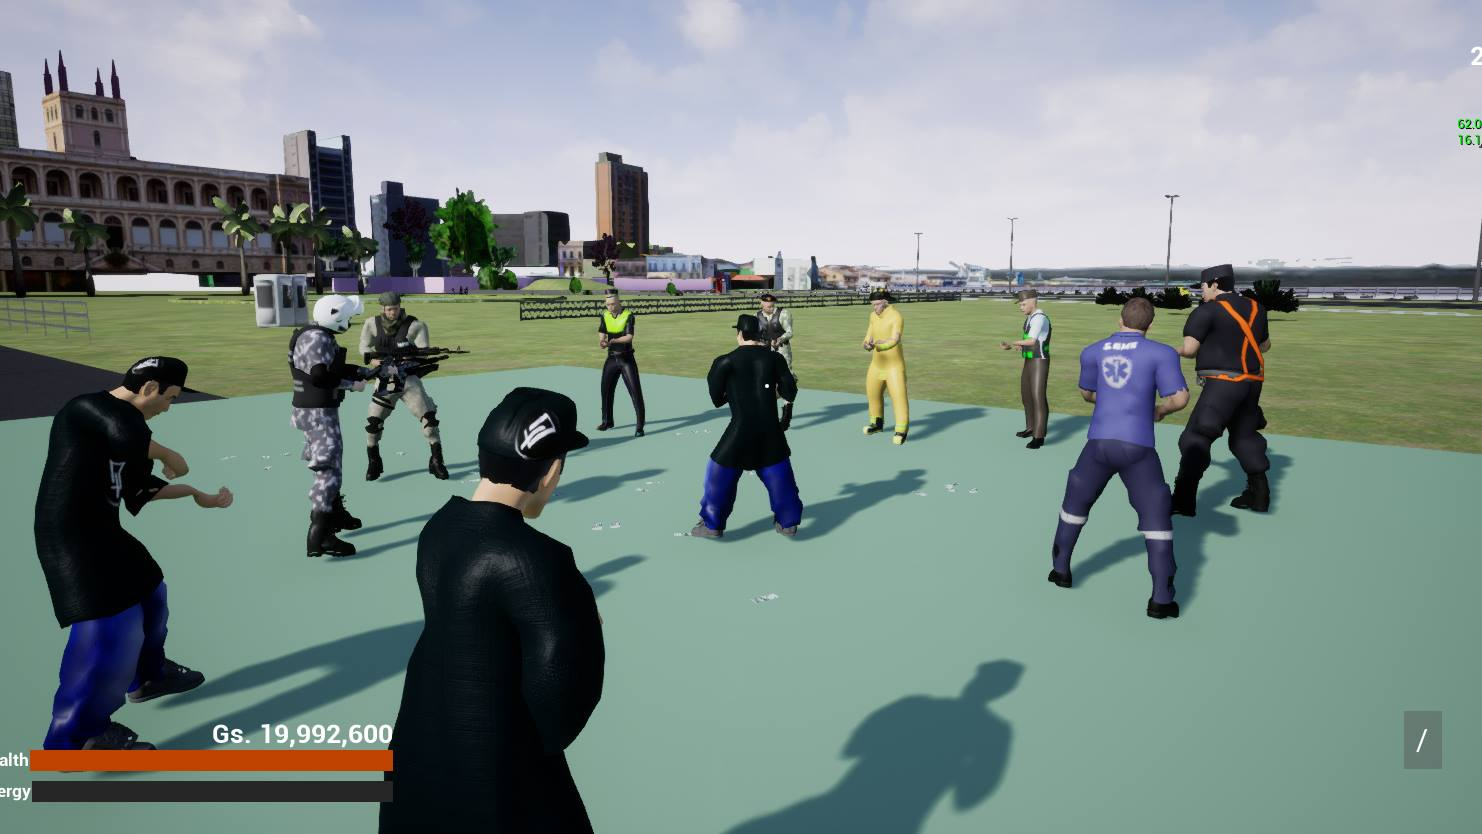
\includegraphics[width=\textwidth]{81.jpg}

  \pagenumbering{arabic}

  \newpage
  \section{Introduction}
  In the proccess for aquire knowledge at some point of our life we need to share the knowledge.
  This is a technical book intended to describe the proccess of making a game. My own game, for aquire technicals habilities

  "Do one thing, and do it well"

  "Make it simple"

  \newpage
  \section{The 3D art}
  
  \subsection{Character}
  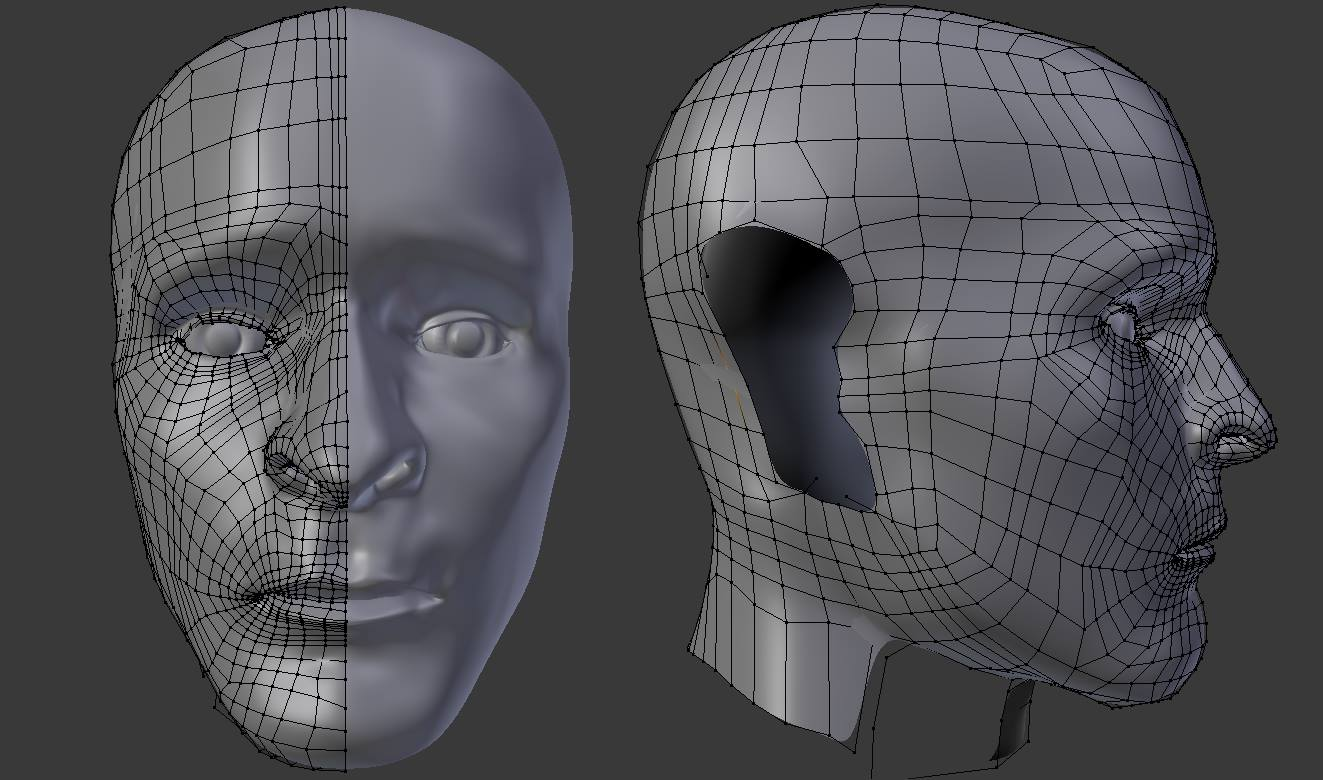
\includegraphics[width=\textwidth]{4.jpg}
  The head was always a challenge


  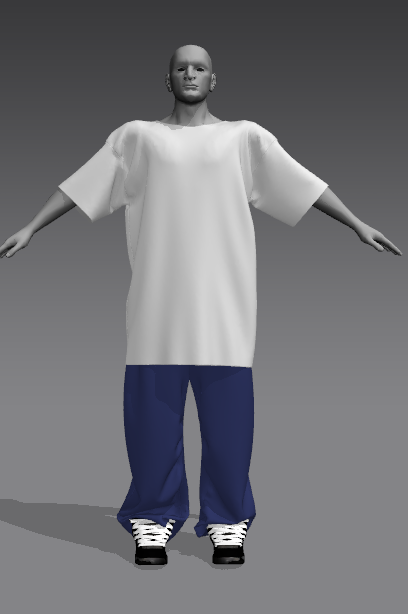
\includegraphics[width=\textwidth]{3.png}
  I used Marvelous Designer for create the cloth


  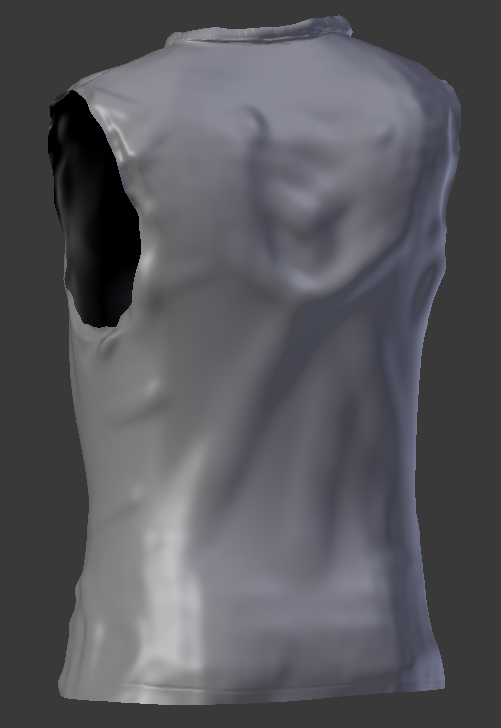
\includegraphics[width=\textwidth]{60.png}
  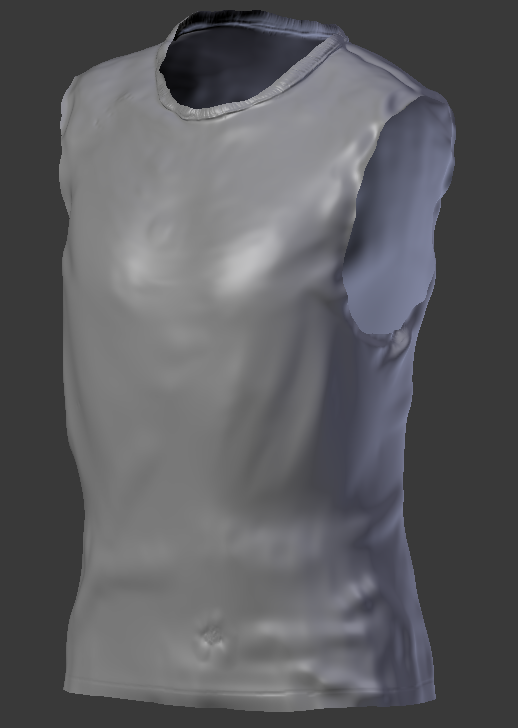
\includegraphics[width=\textwidth]{61.png}
  And i used Blender too, those image show an hightpoly mesh while sculping details in Blender Sculp mode. After you finish your hightpoly you need to do the retopology.

  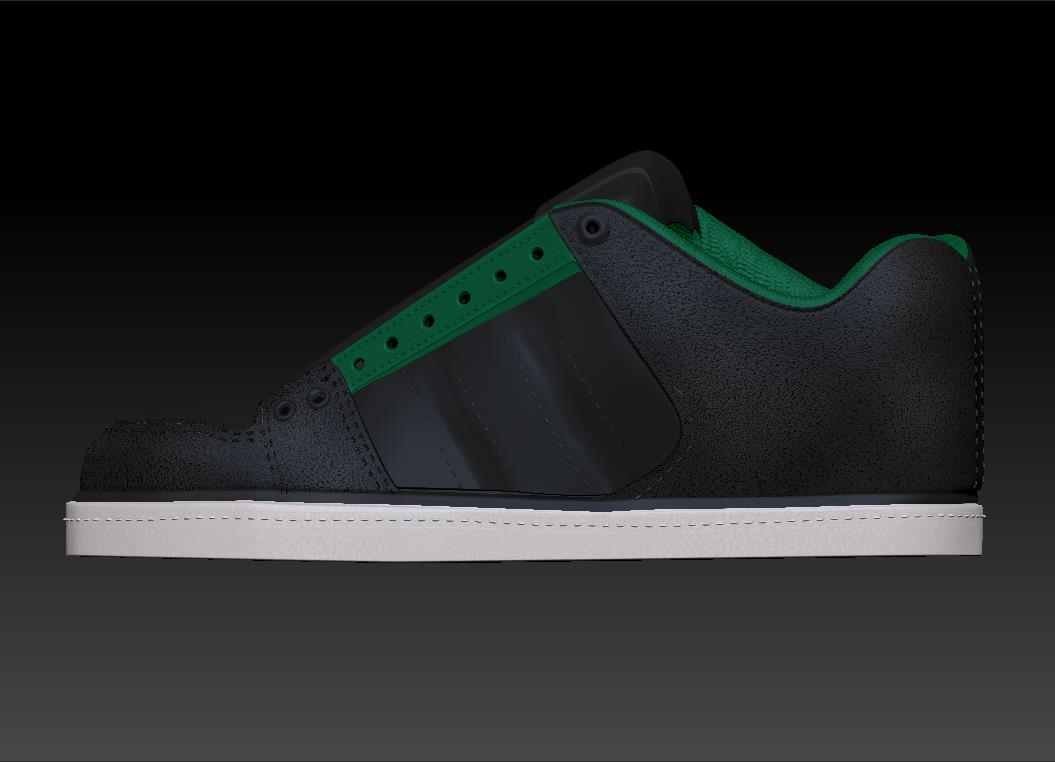
\includegraphics[width=\textwidth]{5.jpg}
  This is in ZBrush for adding details to the shoe

  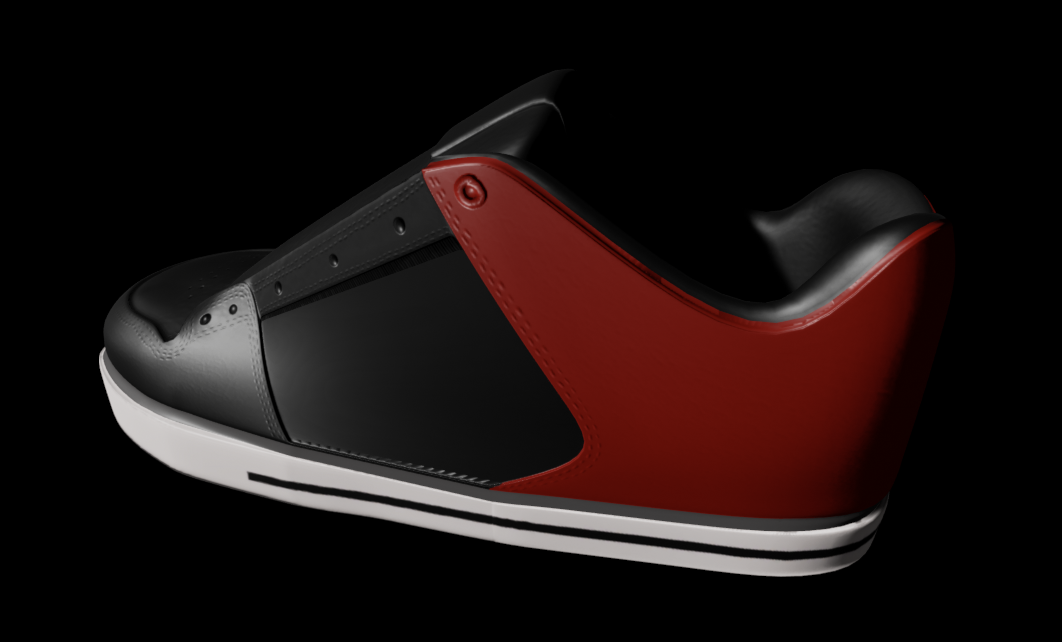
\includegraphics[width=\textwidth]{19.png}
  Do some normals texture from your hightpoly mesh of ZBrush, unrawp the mesh, do some UVediting and you can put the normal for your model.

  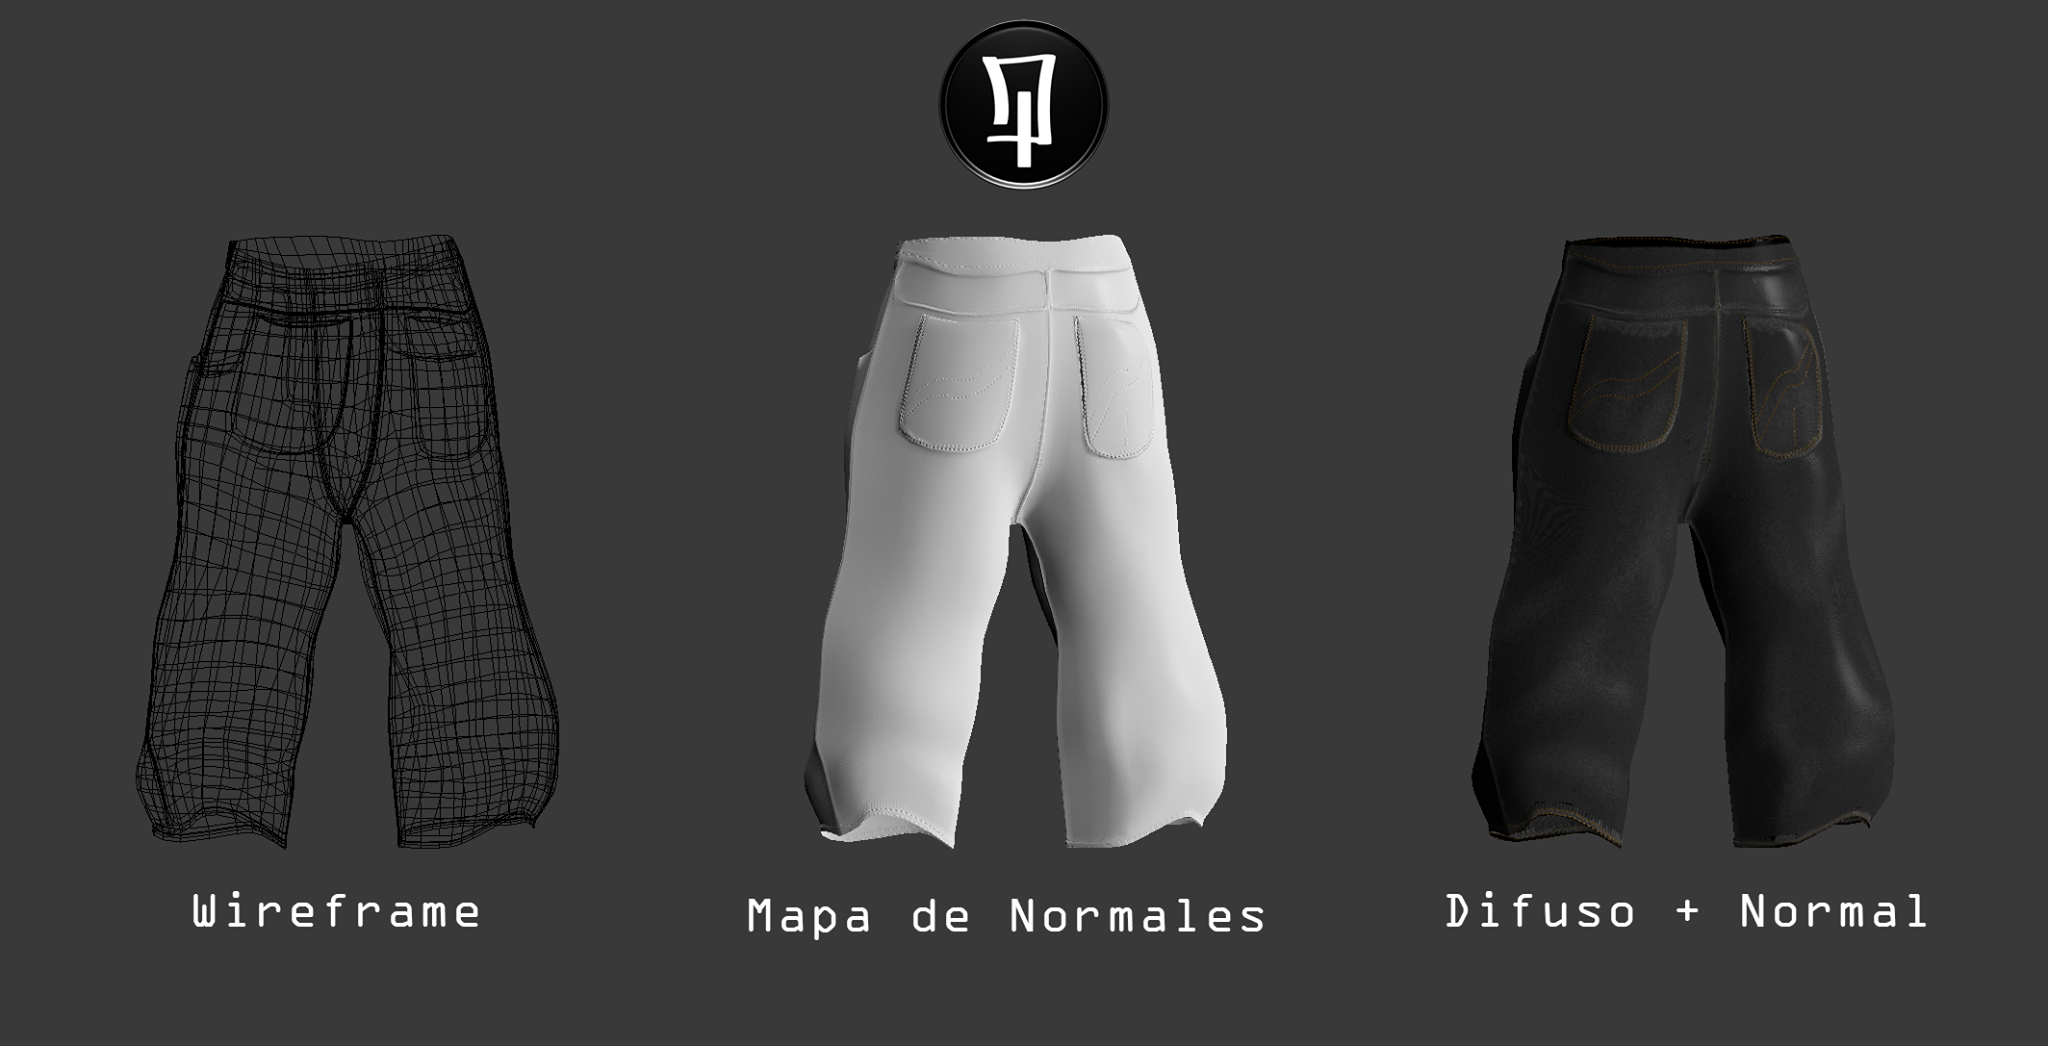
\includegraphics[width=\textwidth]{6.png}
  
  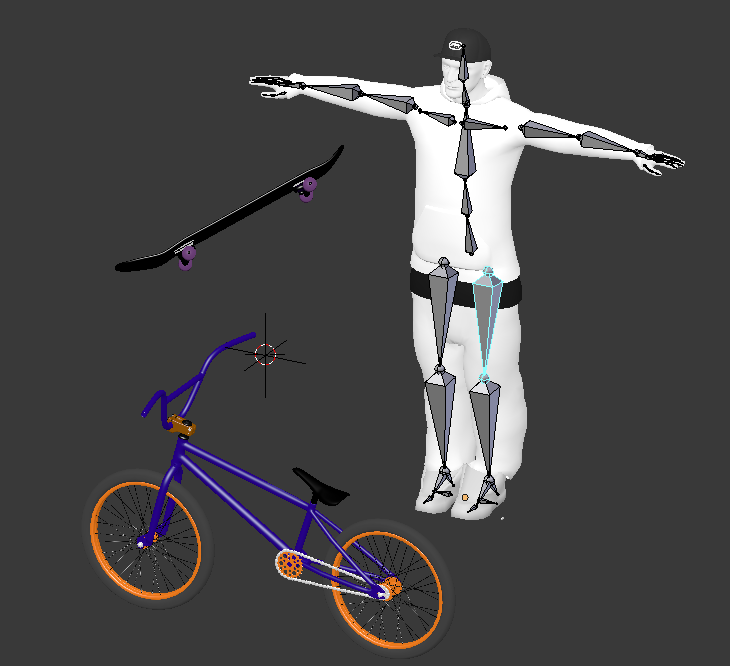
\includegraphics[width=\textwidth]{10.png}
  You need to add skeletal bones on your 3D editor for posing your character

  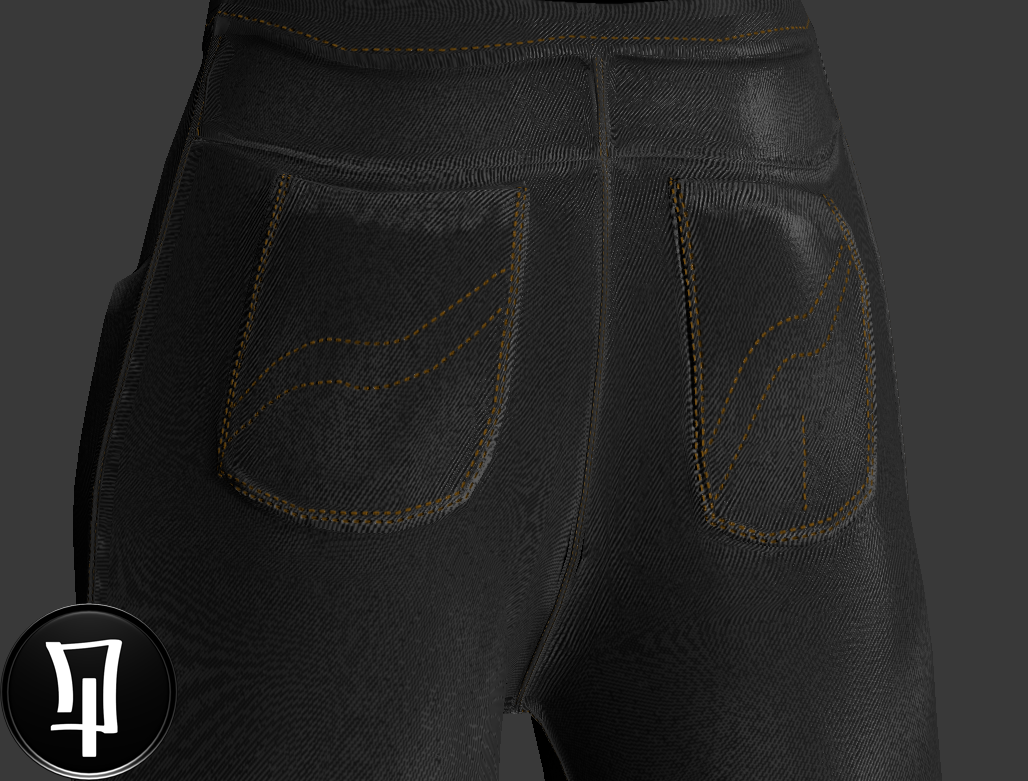
\includegraphics[width=\textwidth]{7.png}
  
  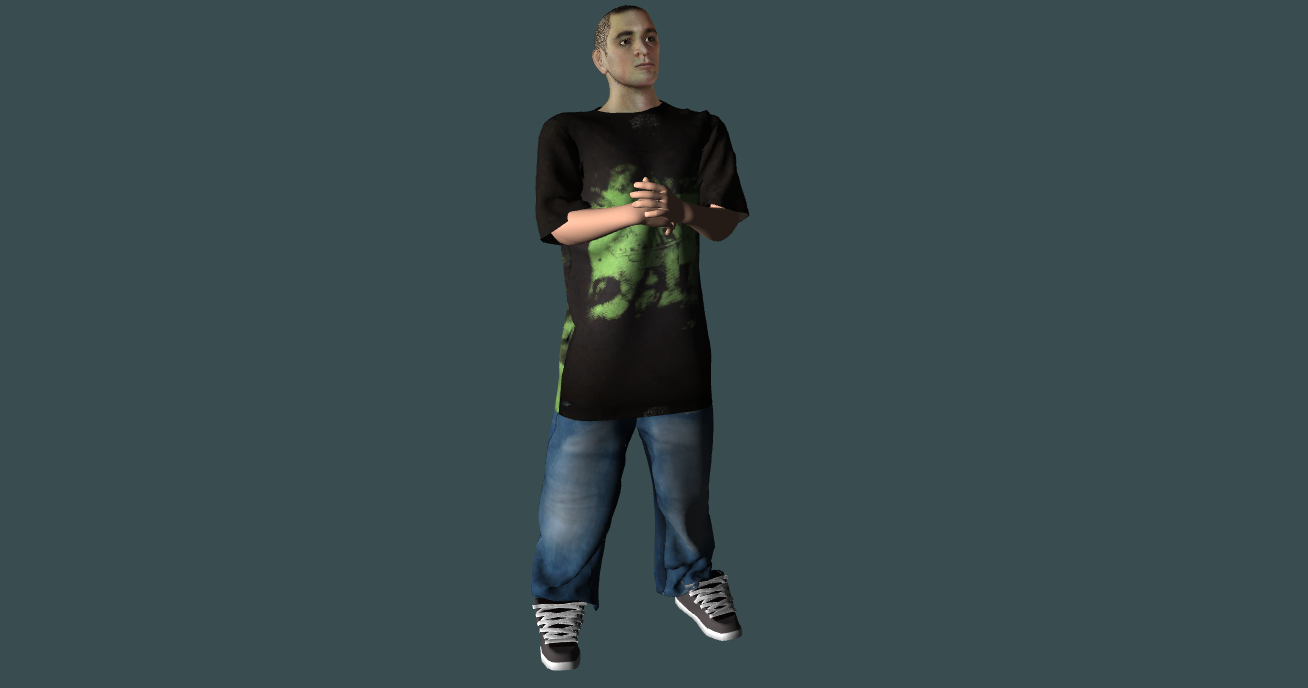
\includegraphics[width=\textwidth]{16.png}
  
  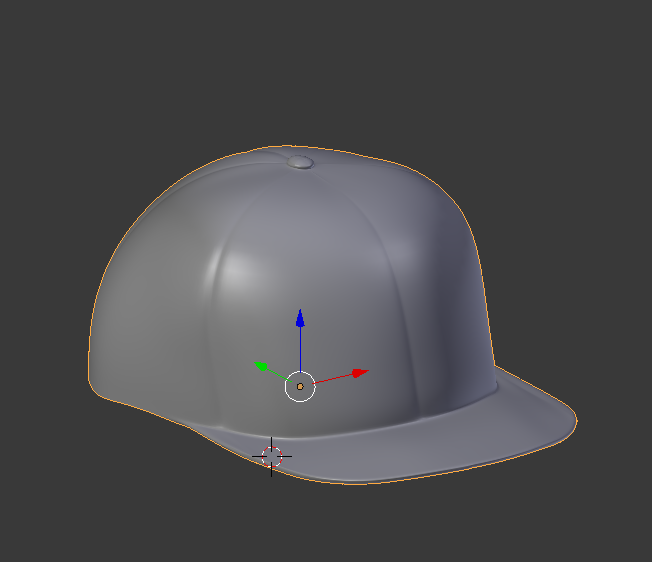
\includegraphics[width=\textwidth]{8.png}
  
  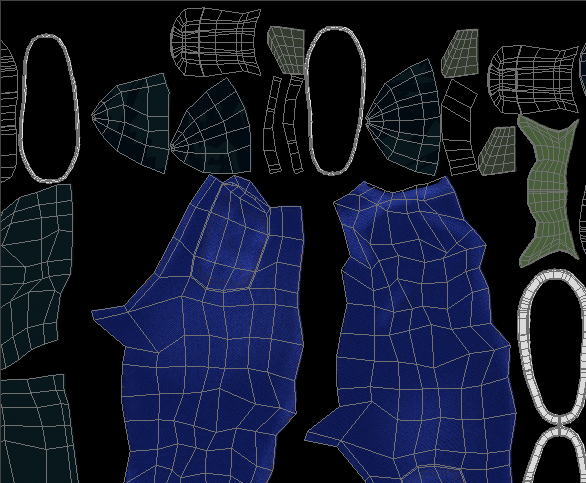
\includegraphics[width=\textwidth]{35.png}
  You can merge all UV like shoes, cloth, skin head in one texture

  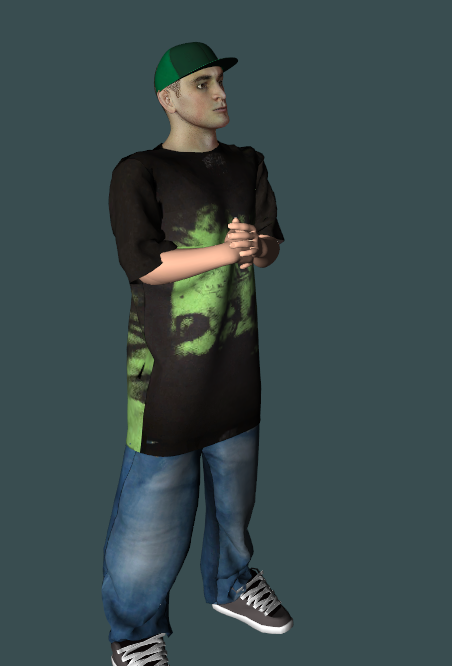
\includegraphics[width=\textwidth]{9.png}
  We have the main character now
  
  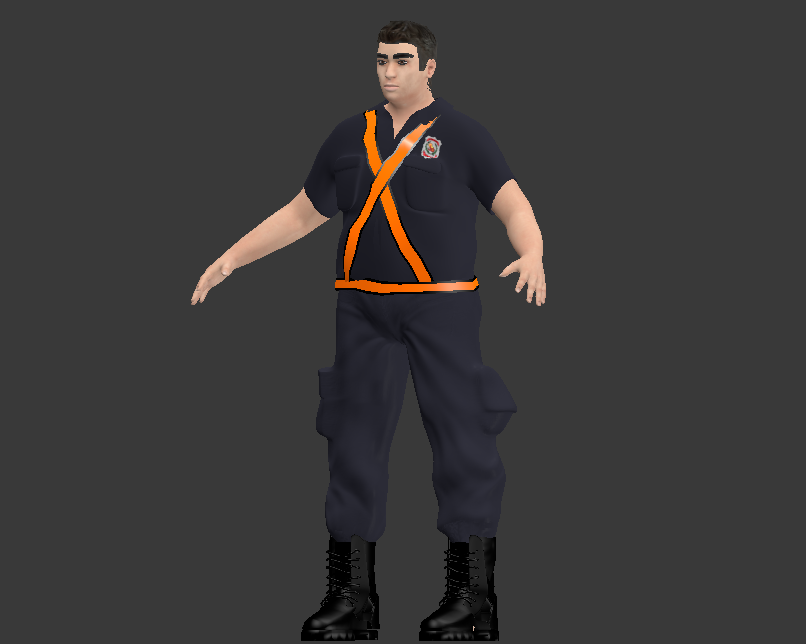
\includegraphics[width=\textwidth]{36.png}
  We need a police man too
  
  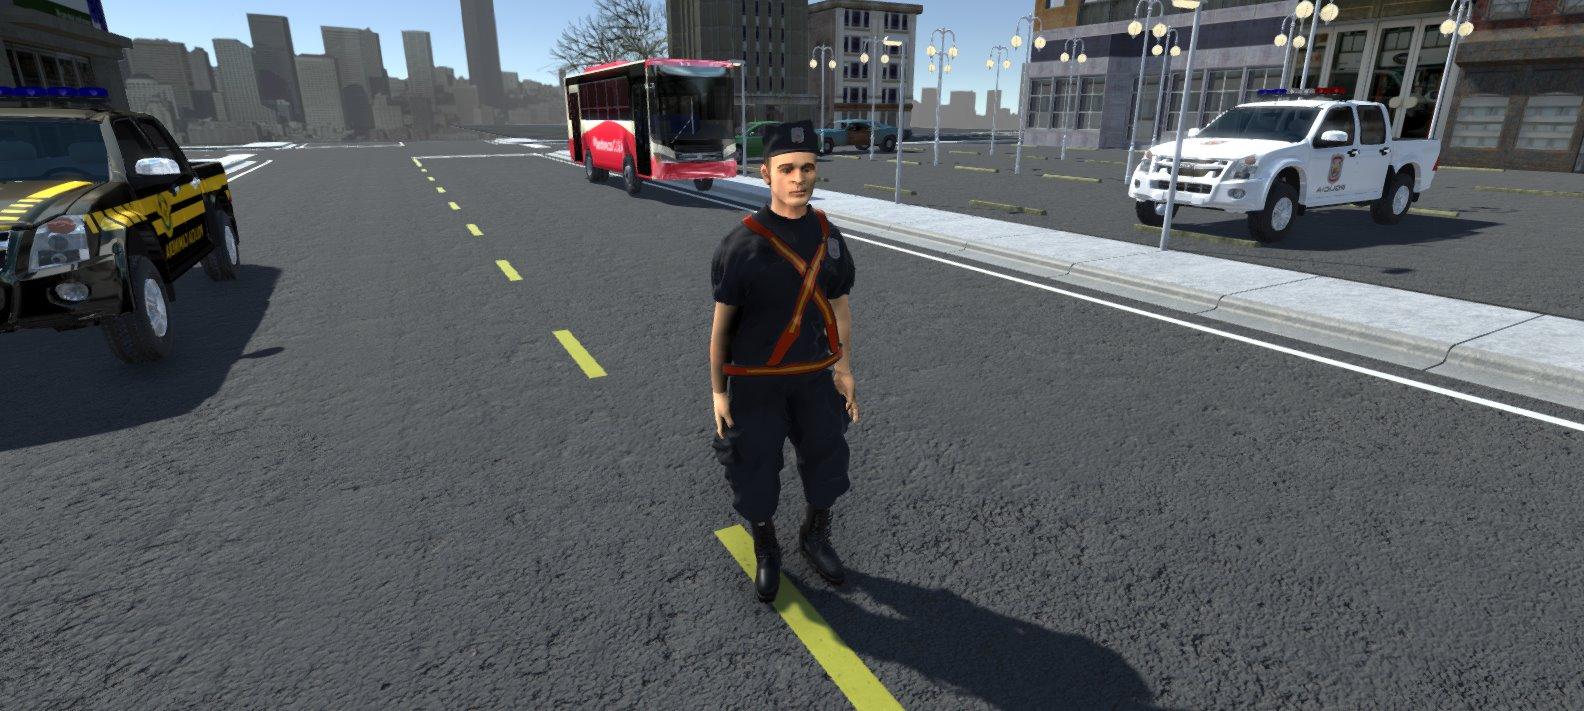
\includegraphics[width=\textwidth]{56.jpg}
  We can custom the main character with "skins"
  
  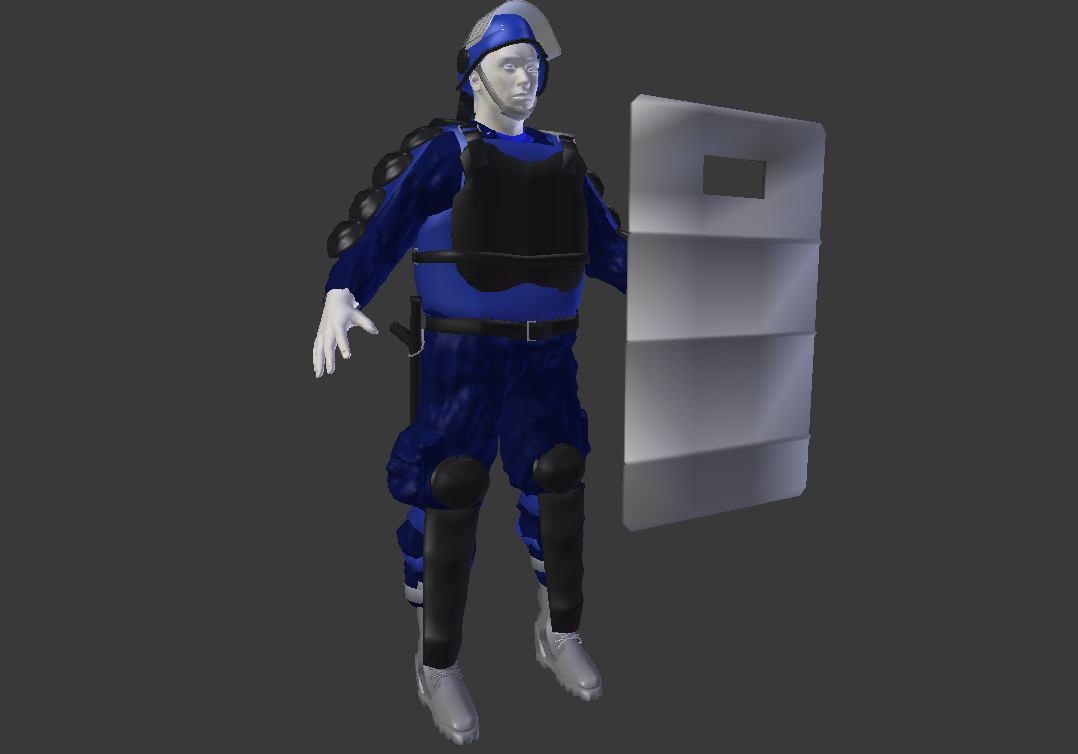
\includegraphics[width=\textwidth]{45.png}

  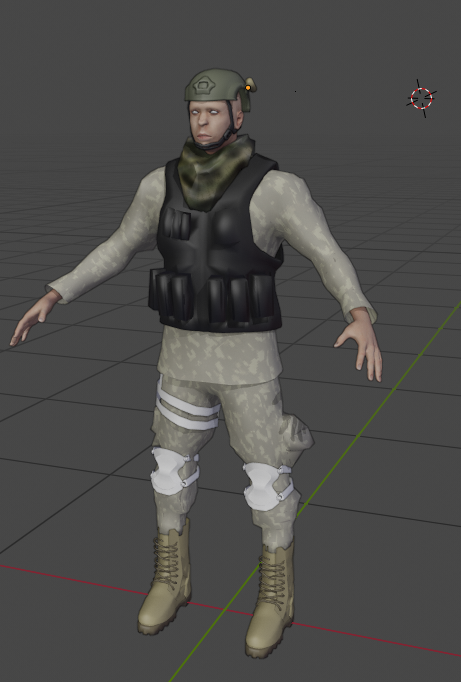
\includegraphics[width=\textwidth]{74.png}

  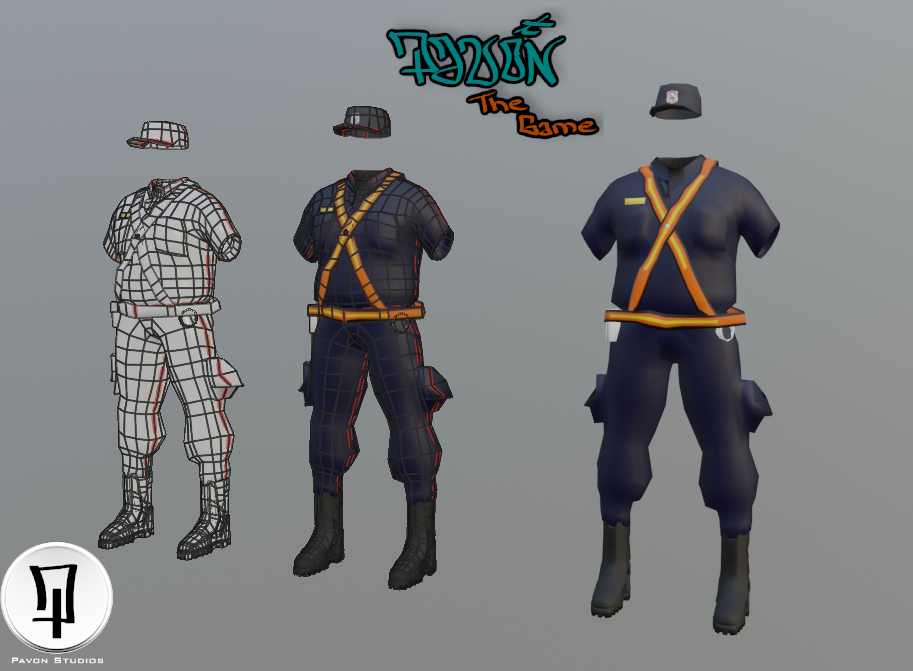
\includegraphics[width=\textwidth]{75.png}

  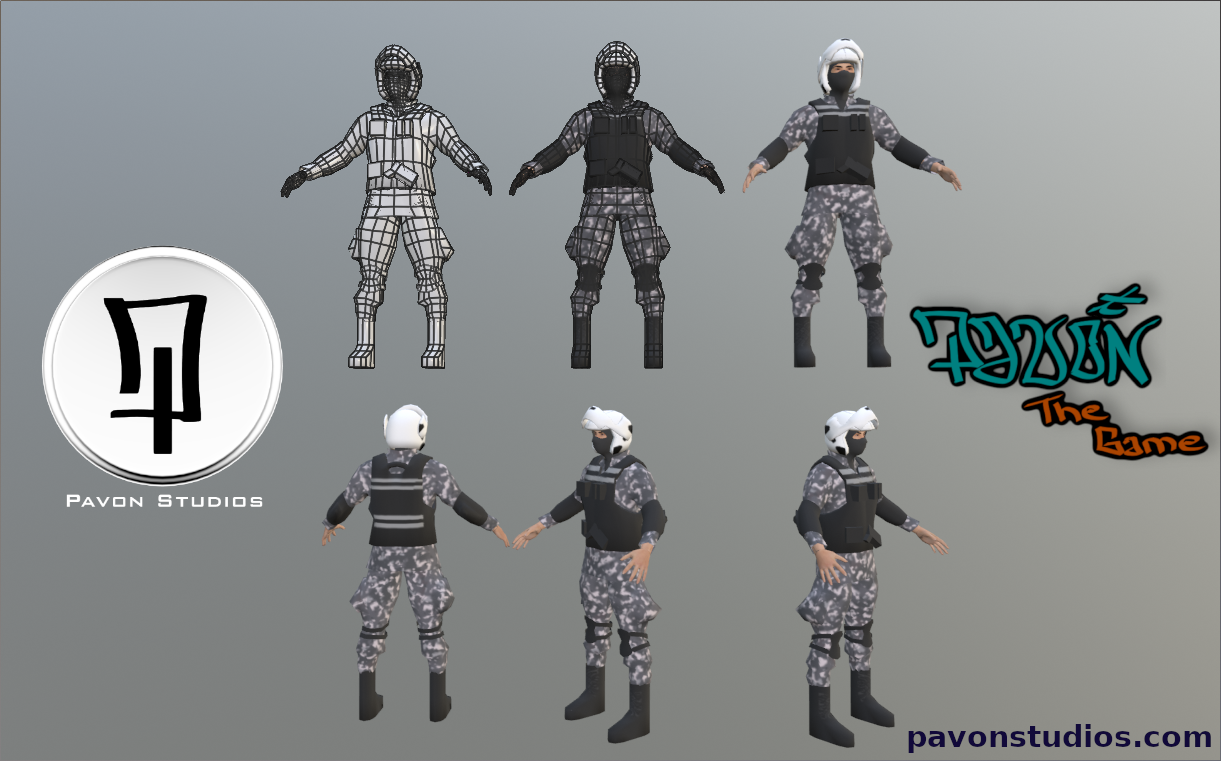
\includegraphics[width=\textwidth]{76.png}

  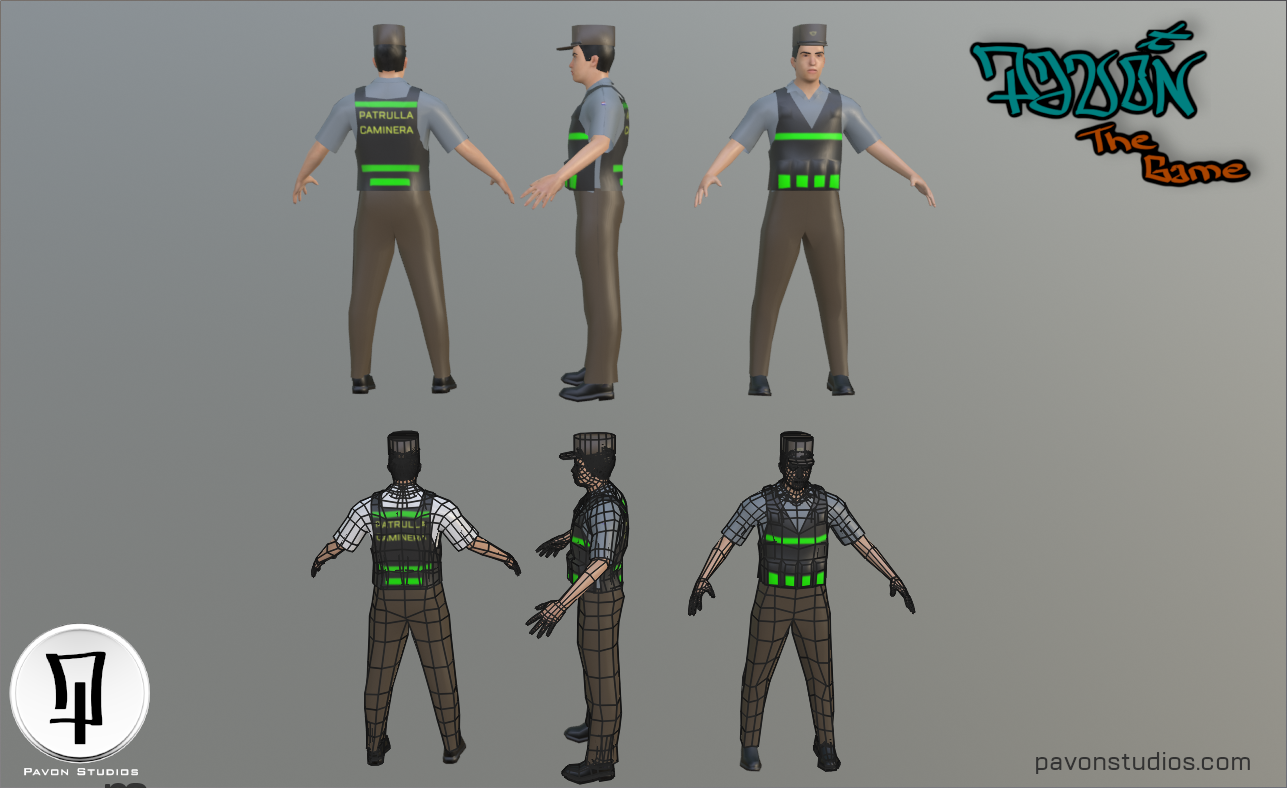
\includegraphics[width=\textwidth]{77.png}

  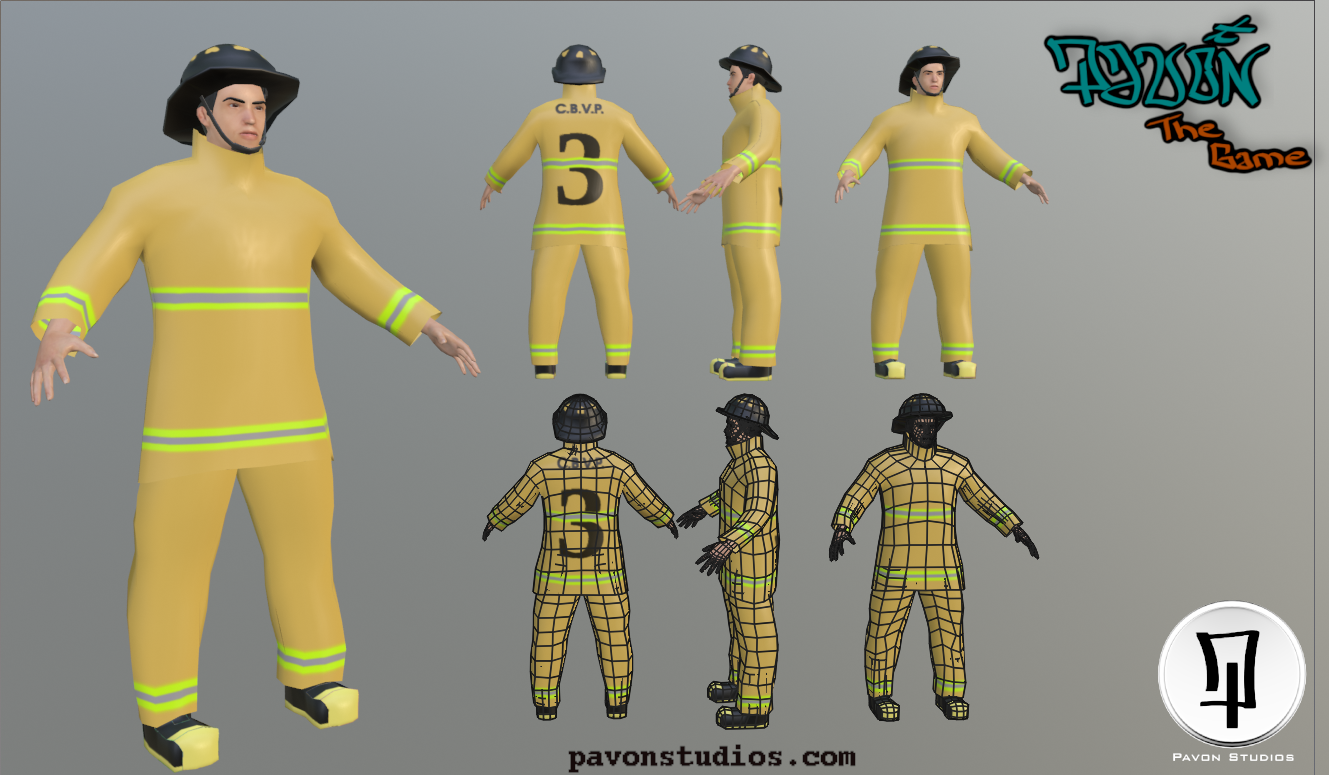
\includegraphics[width=\textwidth]{78.png}

  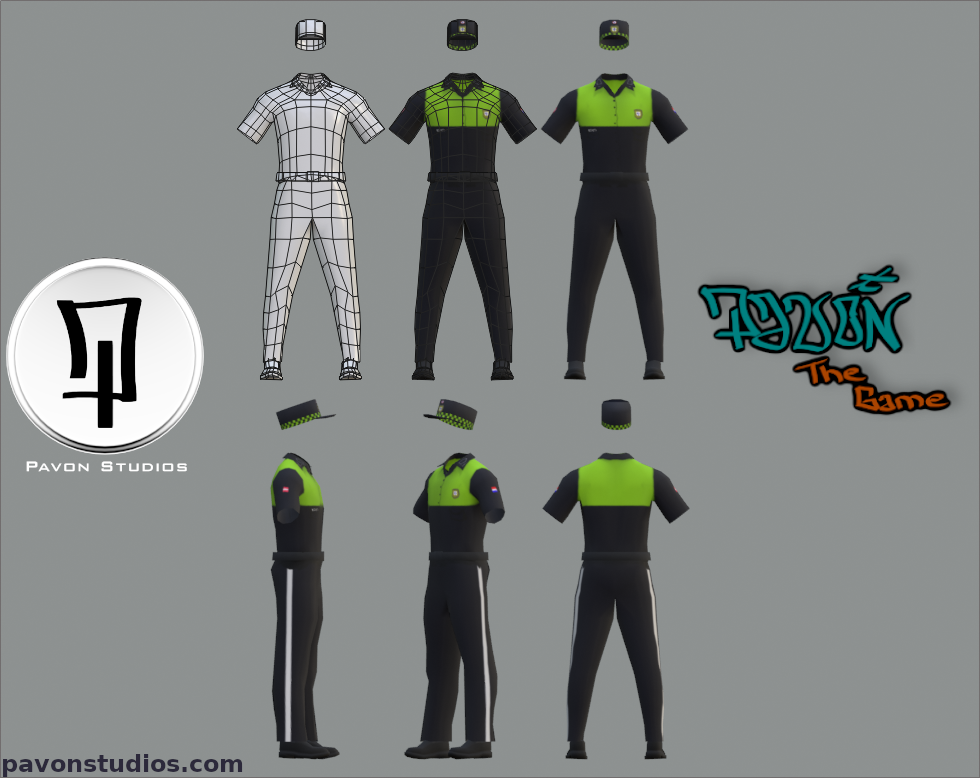
\includegraphics[width=\textwidth]{79.png}

  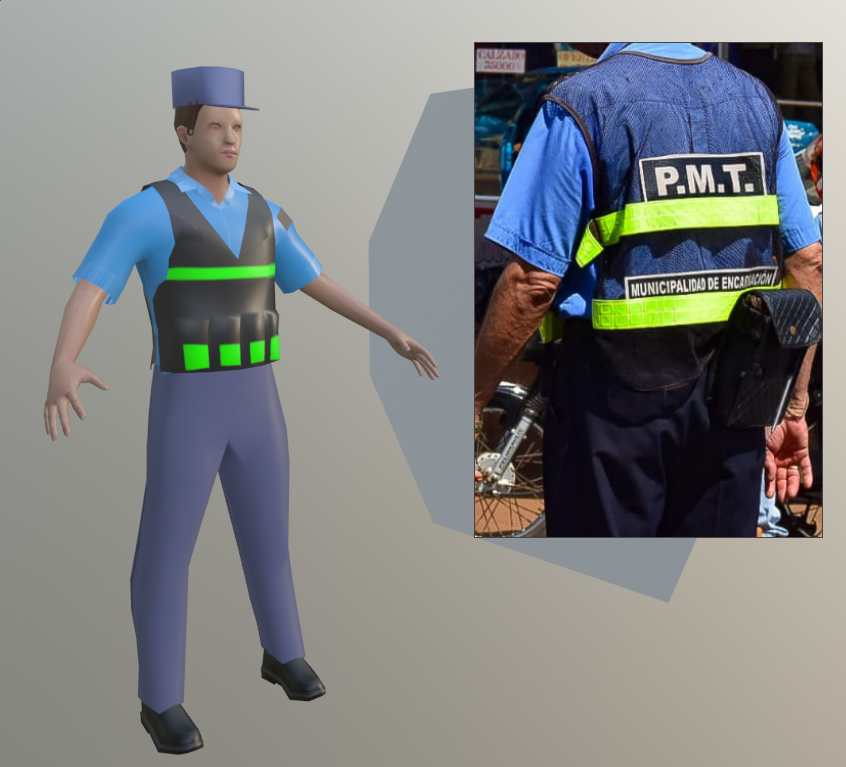
\includegraphics[width=\textwidth]{80.png}

  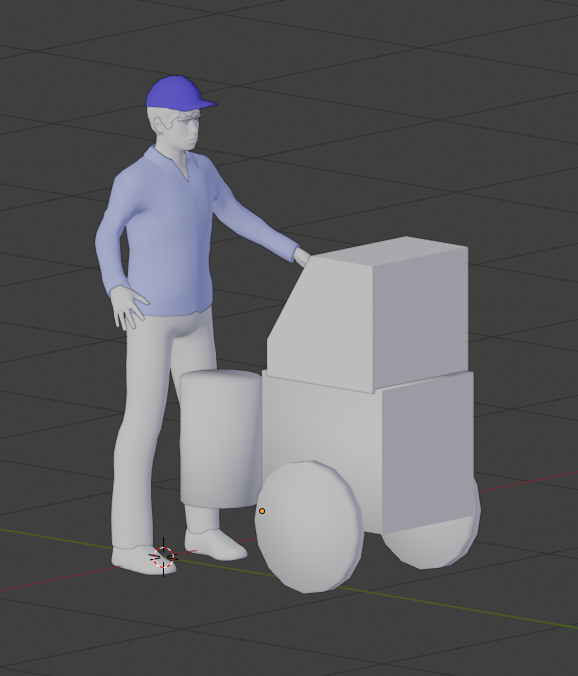
\includegraphics[width=\textwidth]{82.png}

  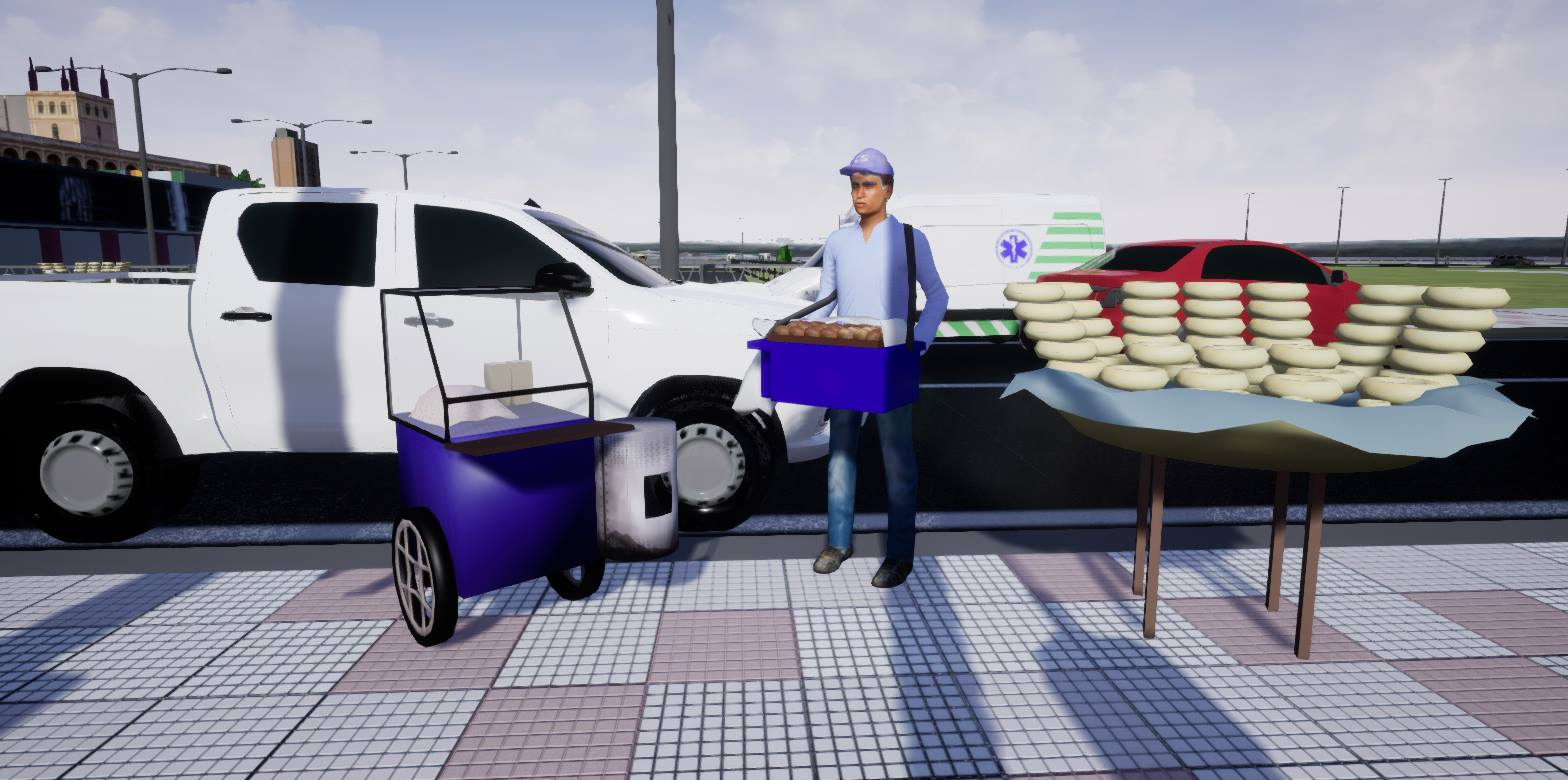
\includegraphics[width=\textwidth]{83.jpg}

  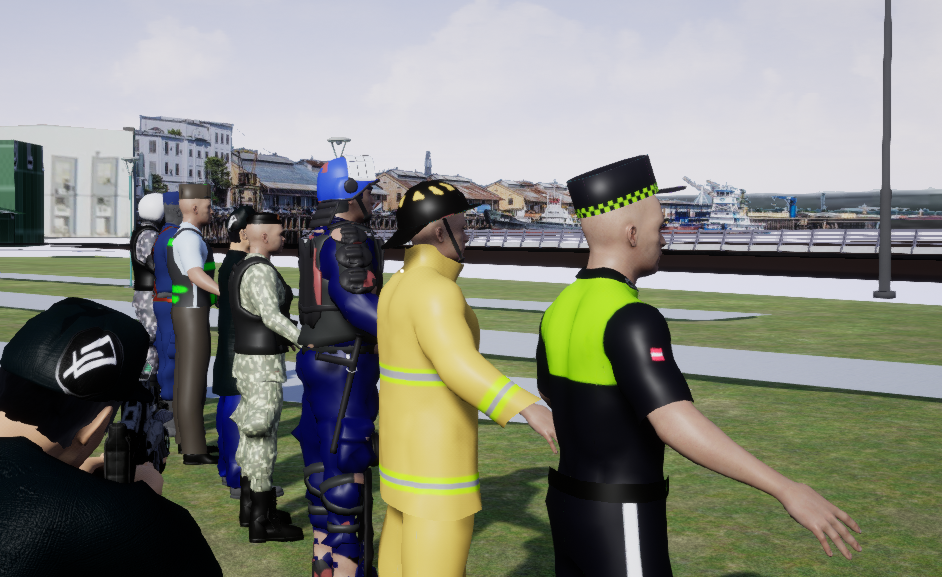
\includegraphics[width=\textwidth]{84.png}

  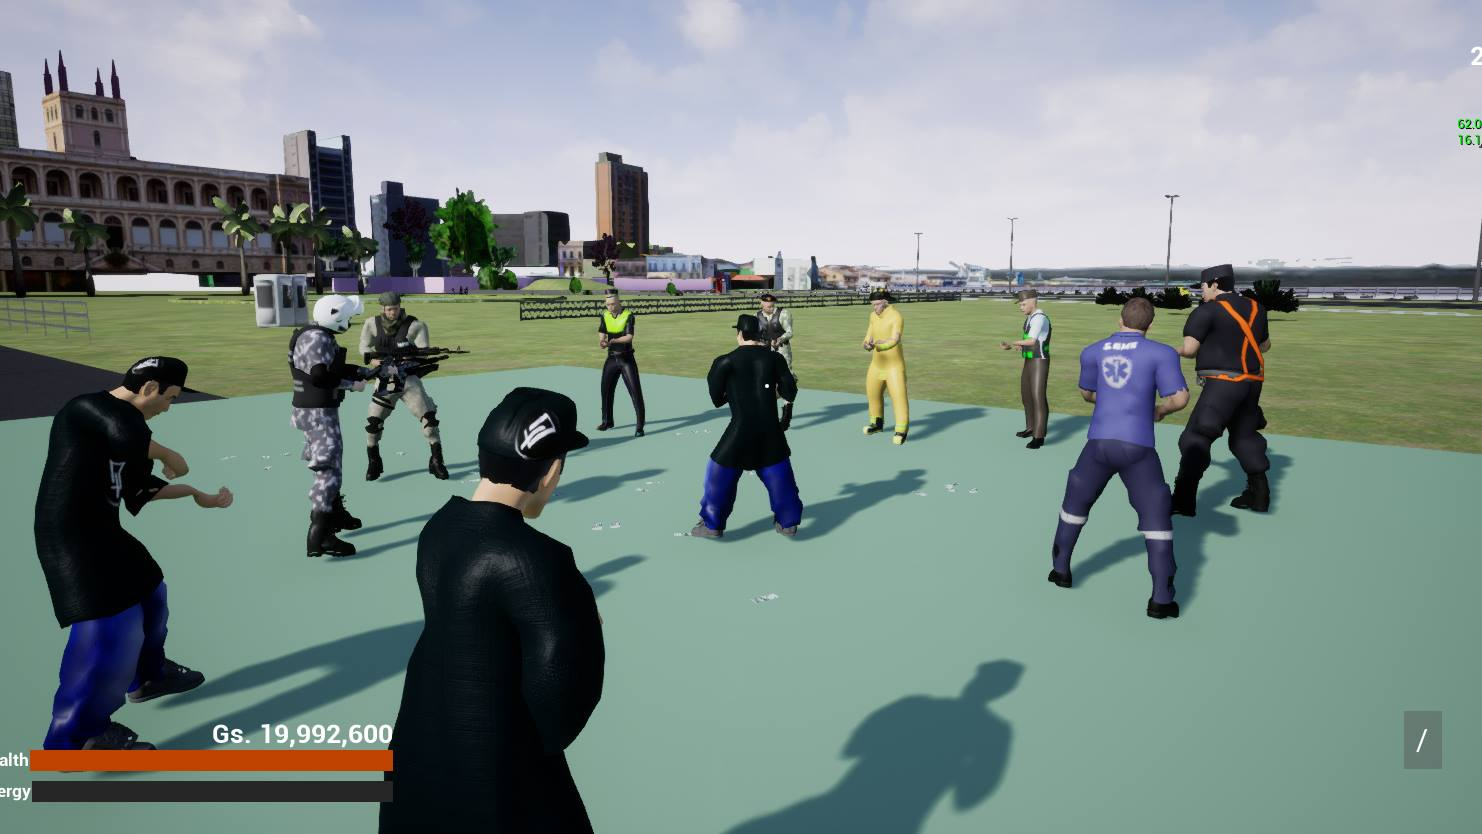
\includegraphics[width=\textwidth]{81.jpg}
  At this point we have many character ready for game play inmertion

  \subsection{Enviroment}
  You will have to create a closed enviroment first because creating a city from scratch take time 
  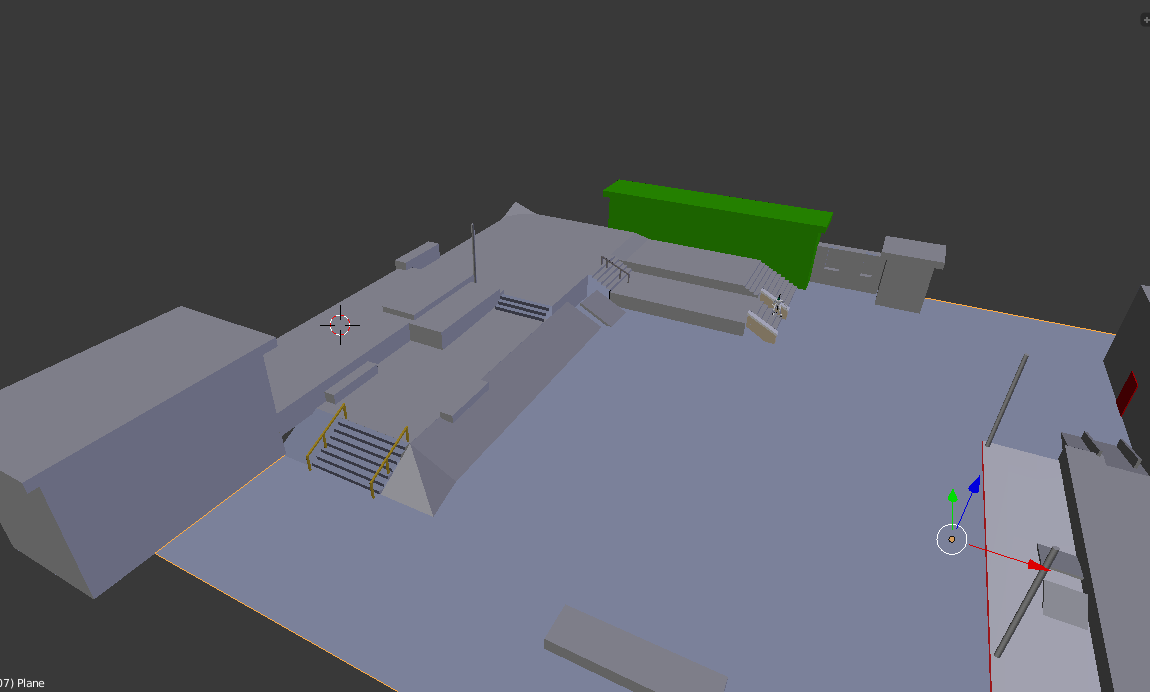
\includegraphics[width=\textwidth]{25.png}
  
  Adding the environment to the game engine and test some ilumination

  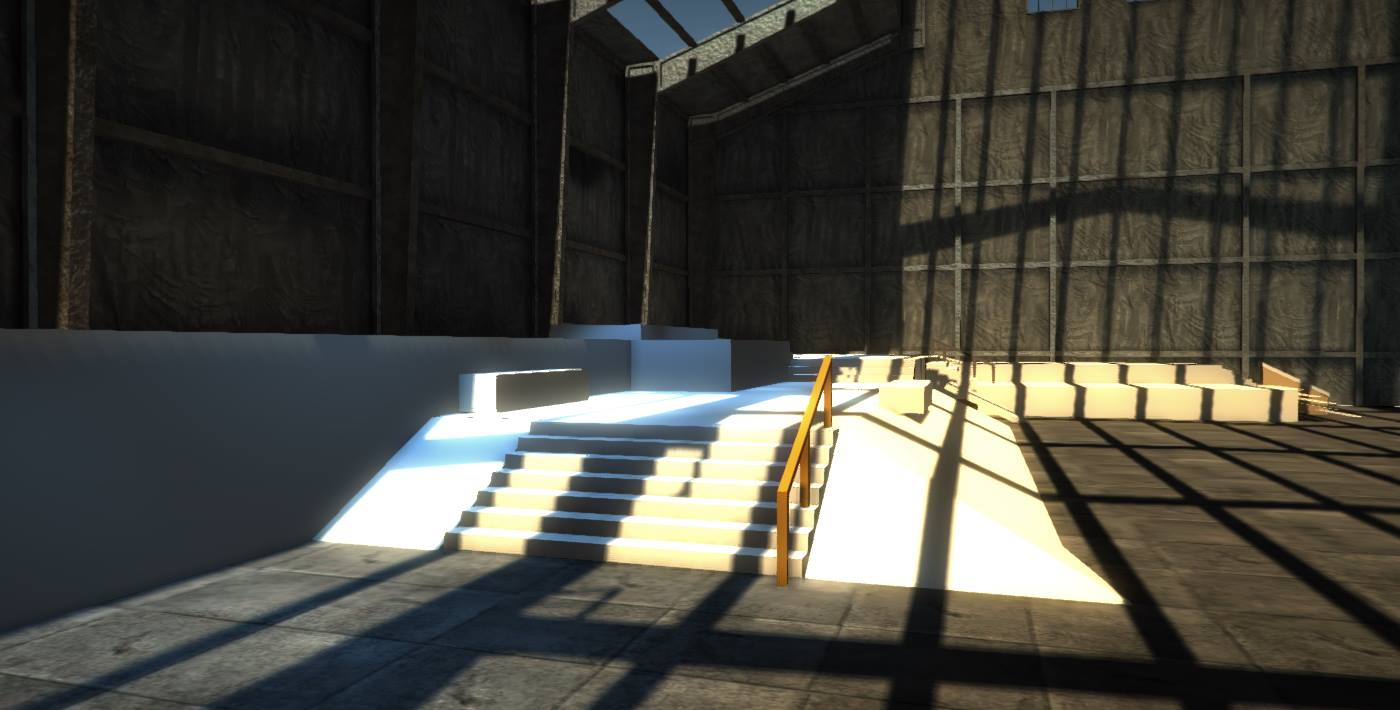
\includegraphics[width=\textwidth]{26.jpg}
  
  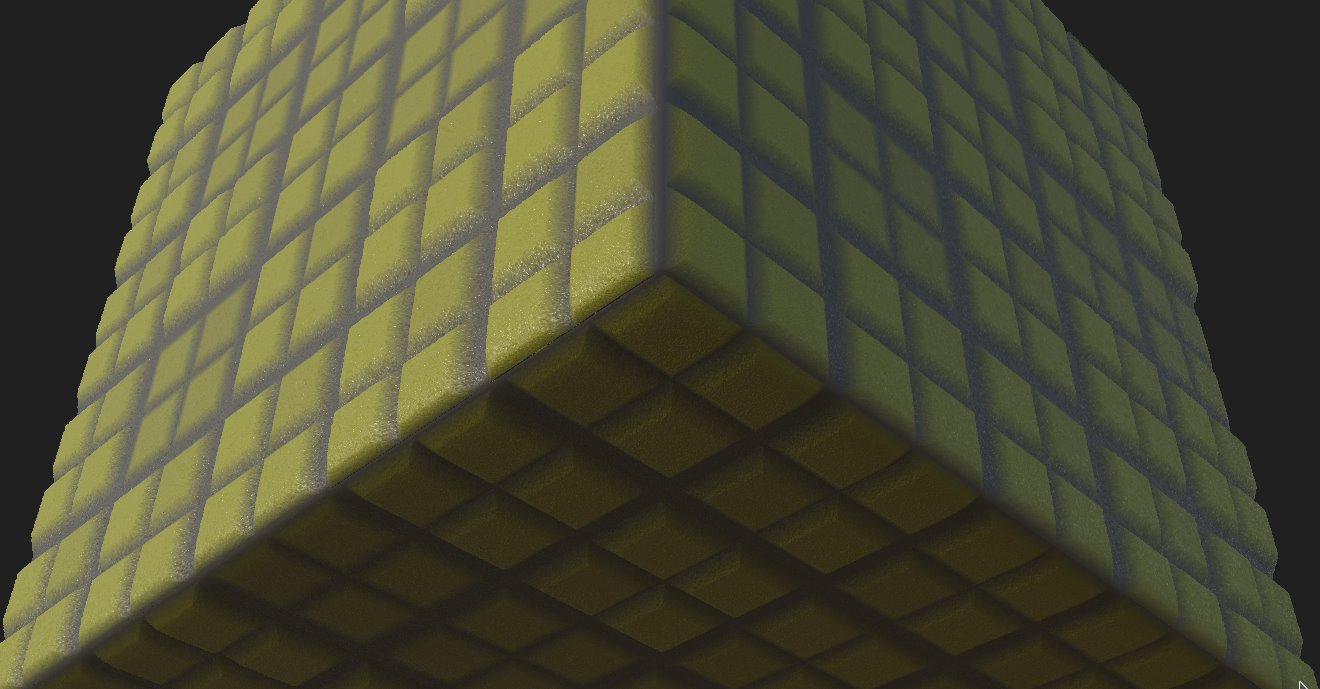
\includegraphics[width=\textwidth]{39.jpg}
  I used Substance for create a procedural tile
  
  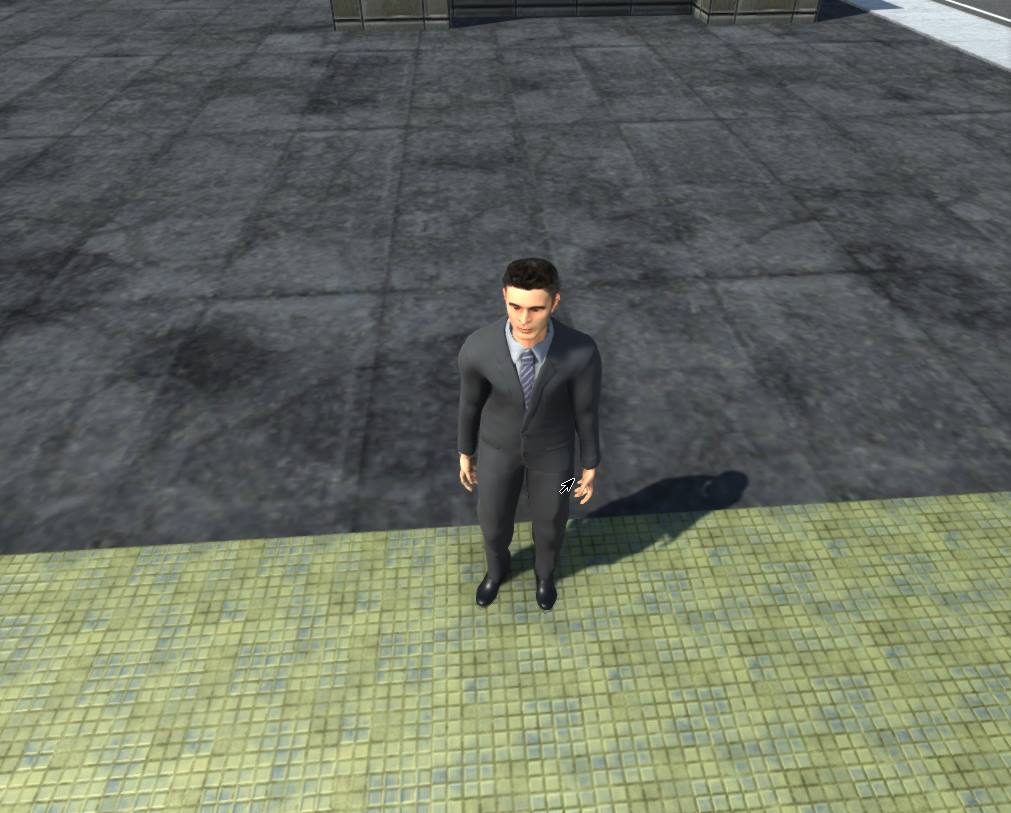
\includegraphics[width=\textwidth]{40.jpg}
  
  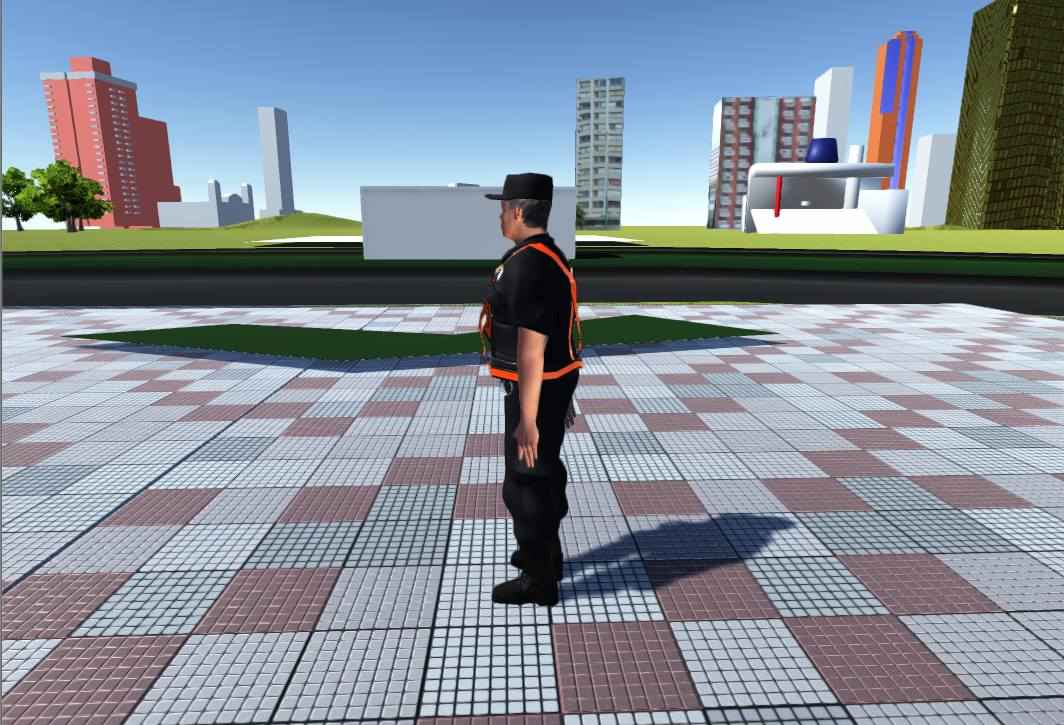
\includegraphics[width=\textwidth]{41.jpg}
  Then i added some color and i got the floor
  
  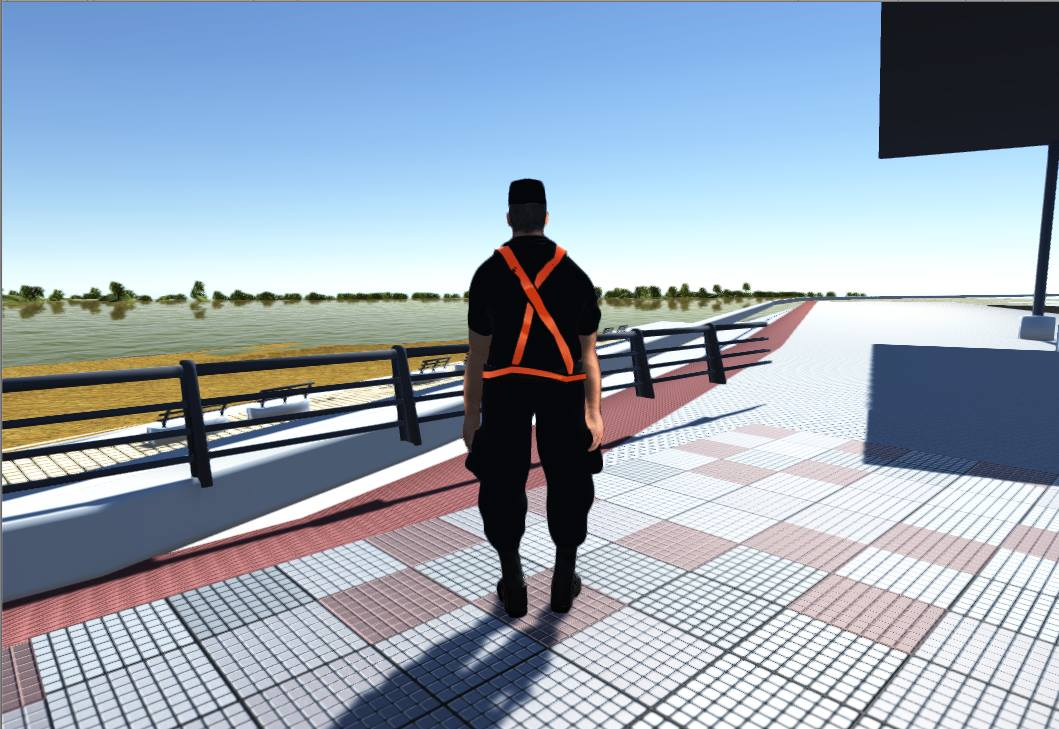
\includegraphics[width=\textwidth]{42.jpg}
  
  \subsection{Vehicles}

  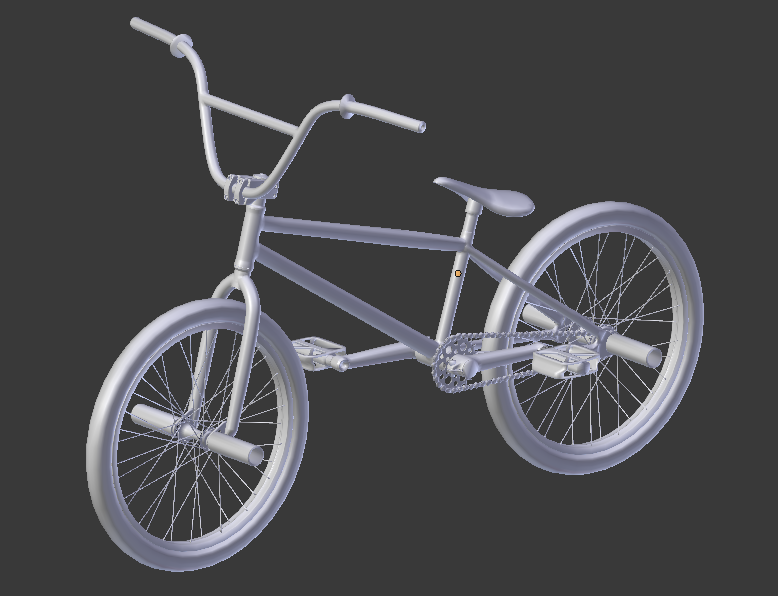
\includegraphics[width=\textwidth]{12.png}

  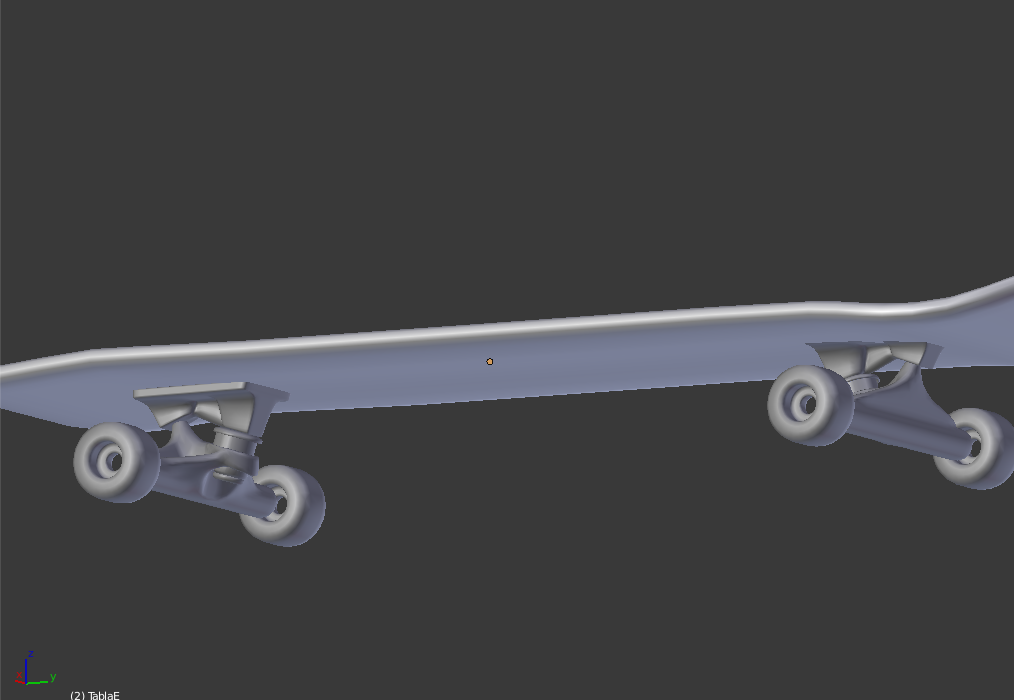
\includegraphics[width=\textwidth]{13.png}
  
  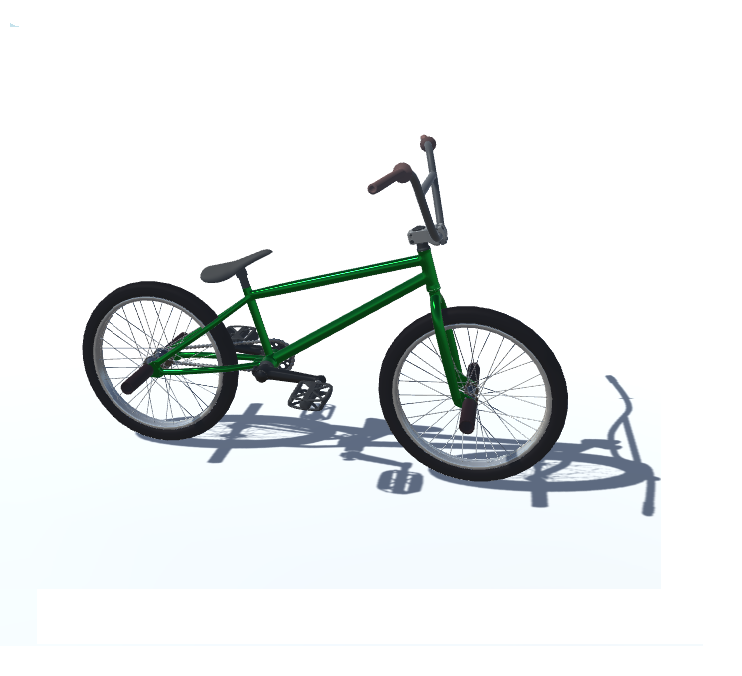
\includegraphics[width=\textwidth]{15.png}

  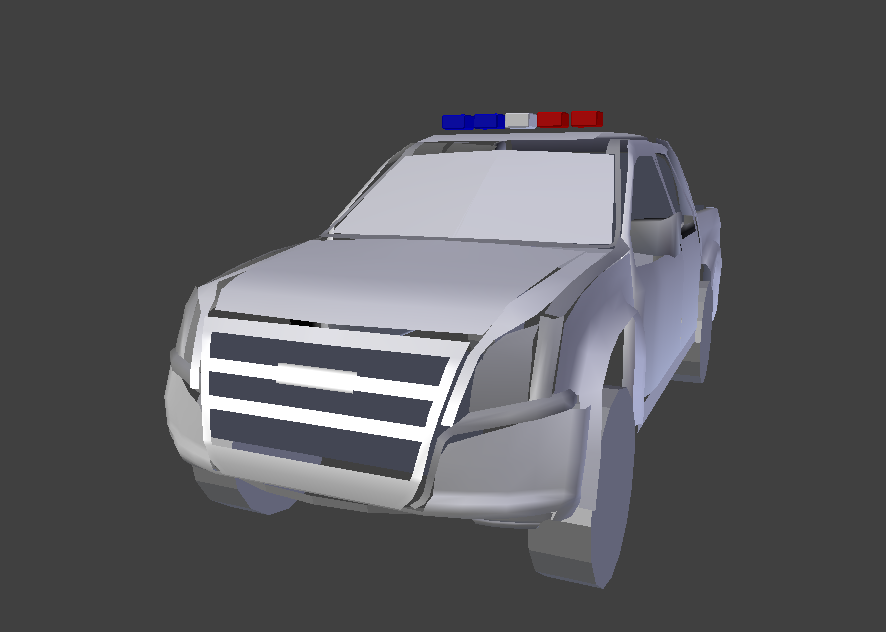
\includegraphics[width=\textwidth]{2.png}
  
  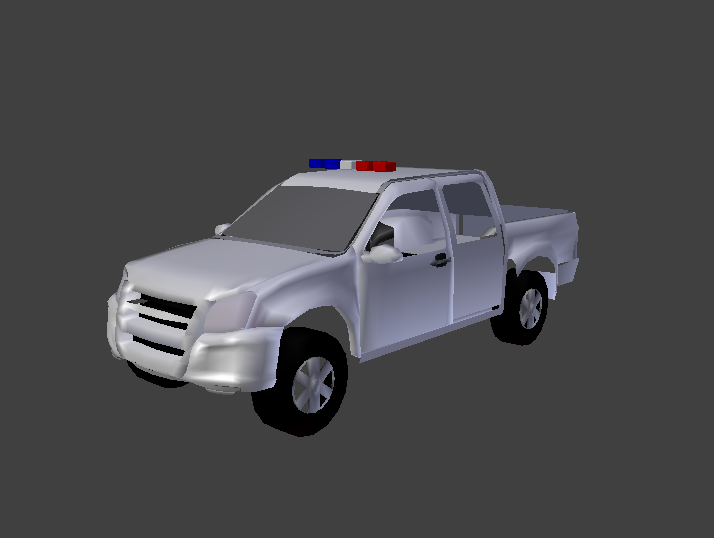
\includegraphics[width=\textwidth]{11.png}

  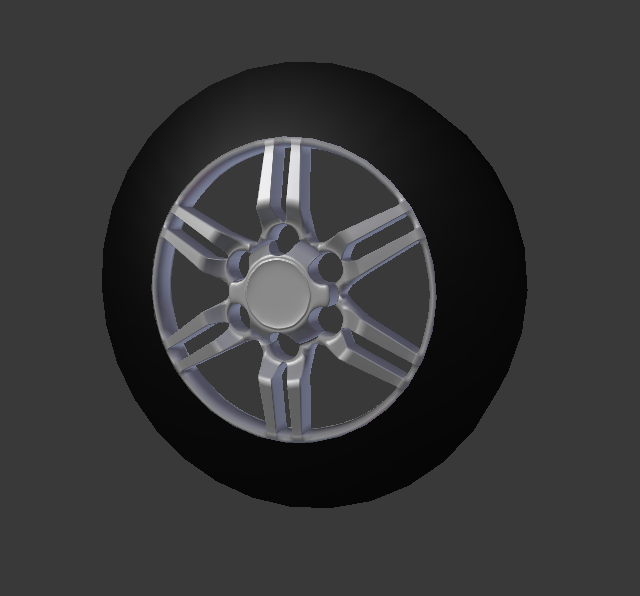
\includegraphics[width=\textwidth]{14.png}

  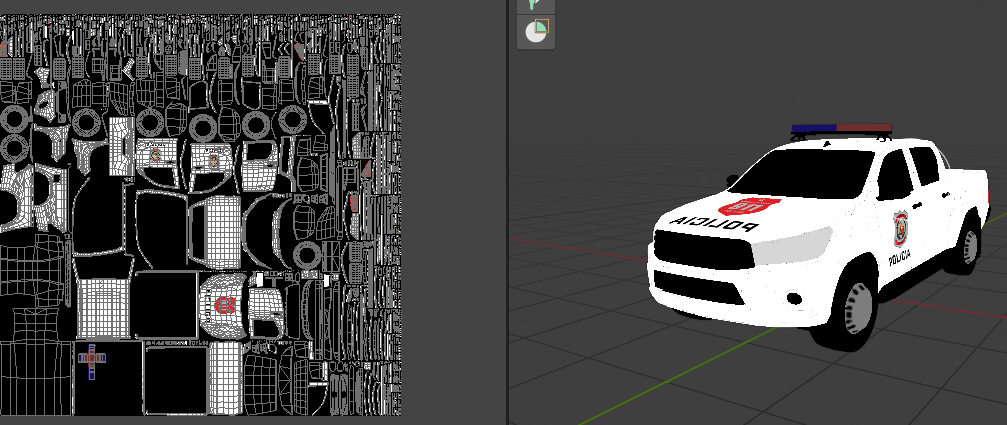
\includegraphics[width=\textwidth]{33.png}

  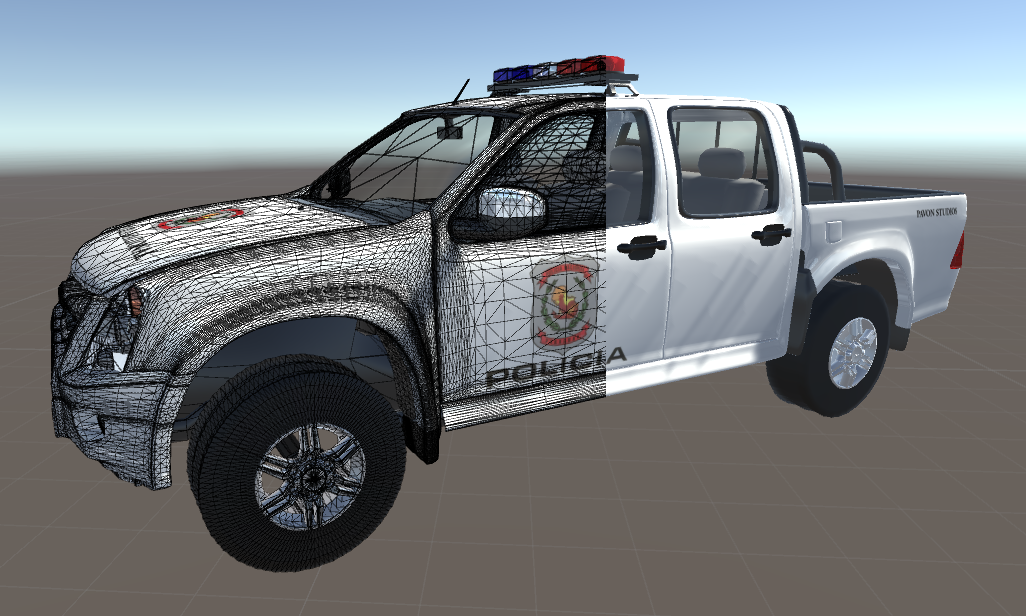
\includegraphics[width=\textwidth]{23.png}
  The proccess of adding textures to a vehicle it's the same of a shoe, but you will be need a 2D Image editor. And of course i used GIMP but also the texture editor of Blender


  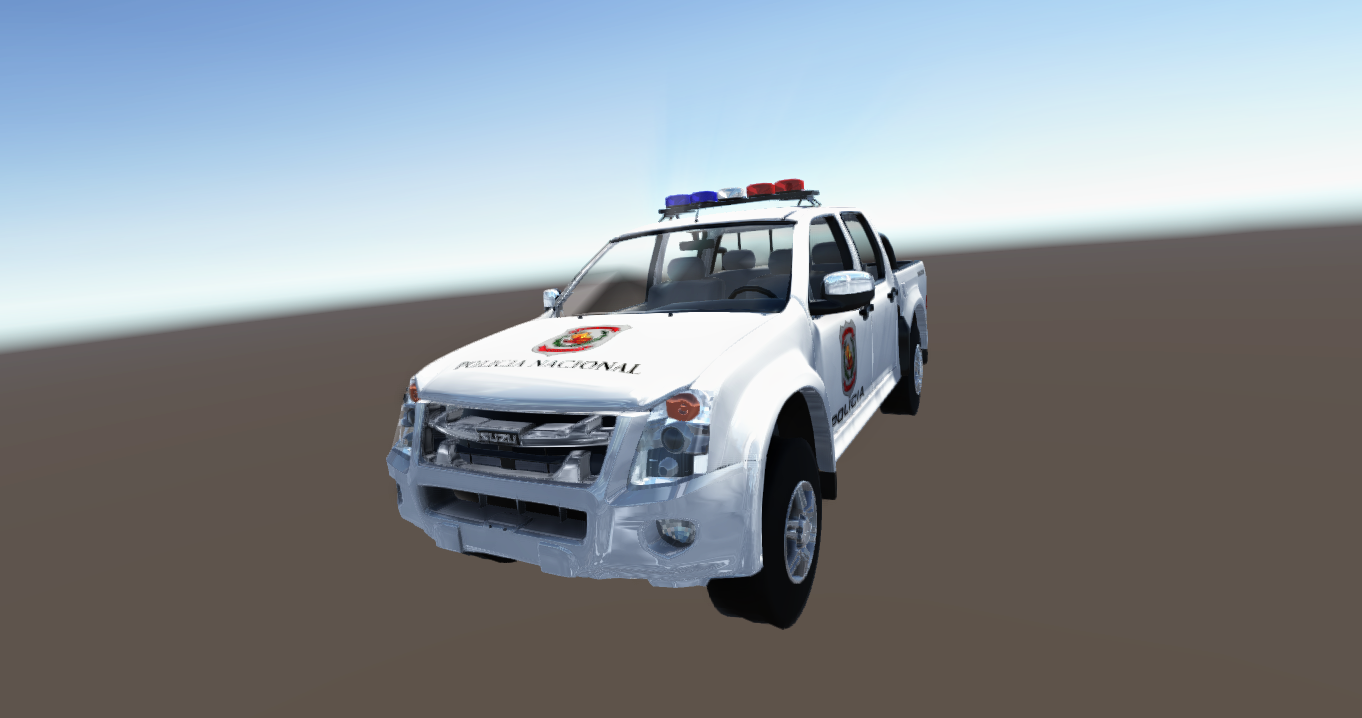
\includegraphics[width=\textwidth]{24.png}
  
  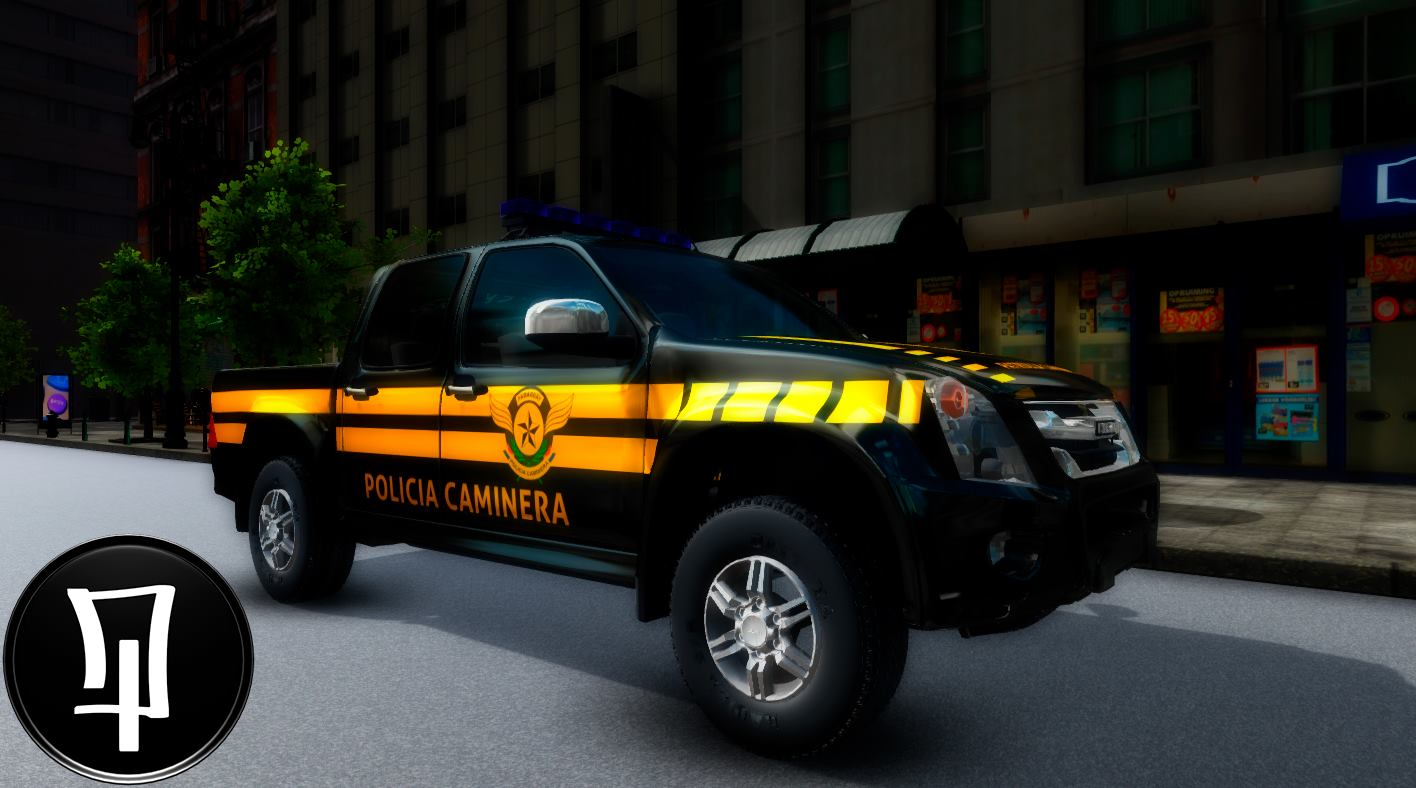
\includegraphics[width=\textwidth]{37.jpg}
  Now we only need to modidier the texture of the model a we have another vehicle
  
  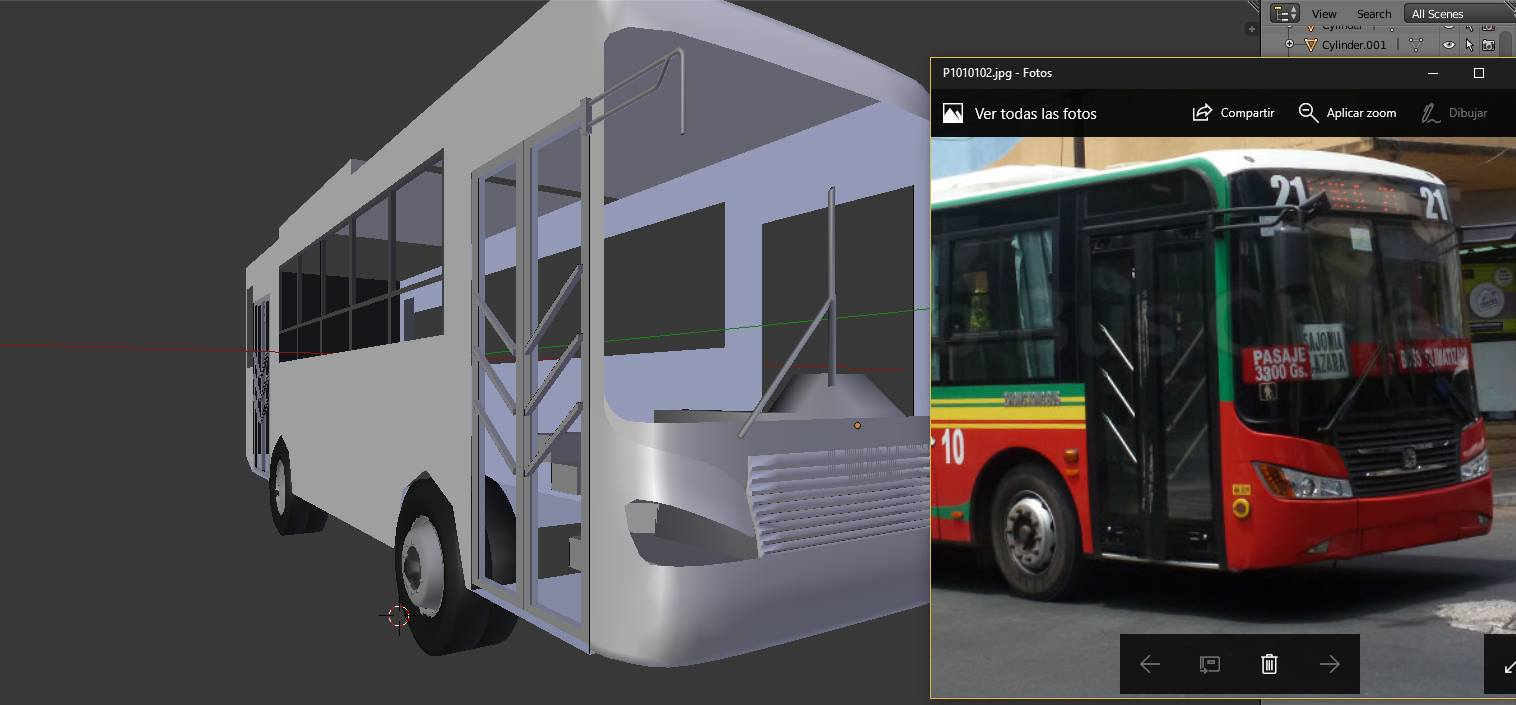
\includegraphics[width=\textwidth]{43.jpg}
  The bus with the reference real image
  
  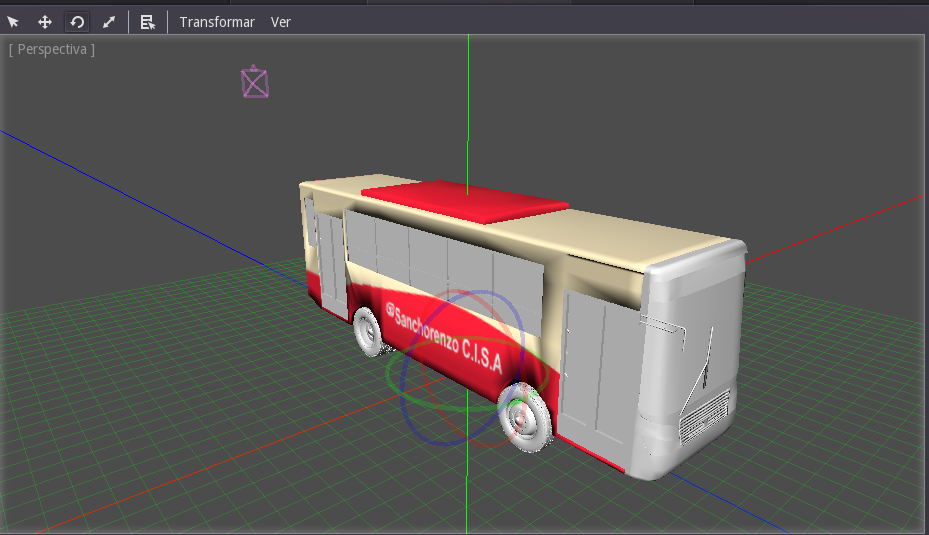
\includegraphics[width=\textwidth]{44.png}


  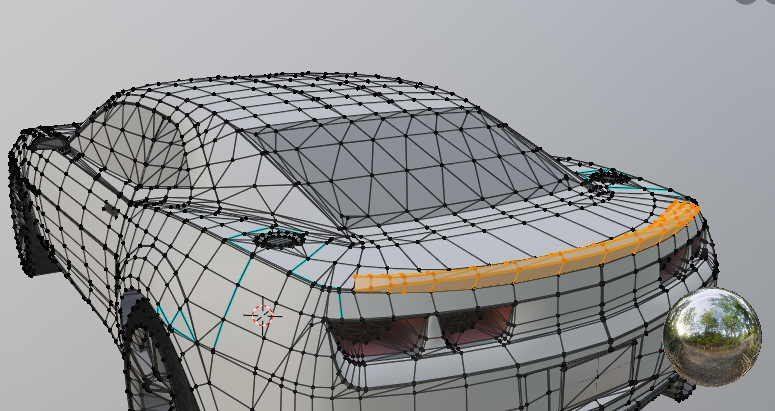
\includegraphics[width=\textwidth]{34.png}
  All proccess of making vehicles at this point are the same, so you can find vehicles from 3D models WebPages and download it. But you will need to do some adjubment anyway. Like changer triangles to quad, create the UV map, simplified the model. Add somed specifics details and so on.
  
  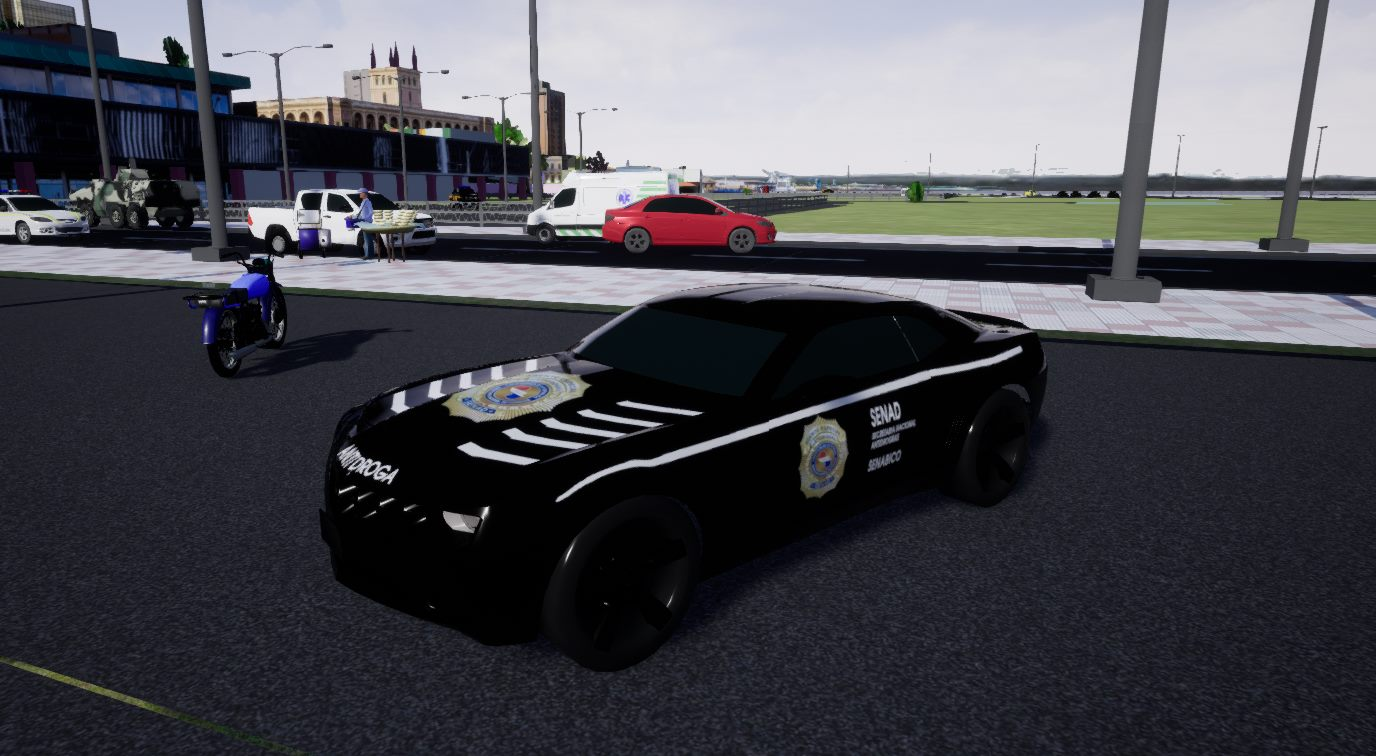
\includegraphics[width=\textwidth]{66.jpg}
  
  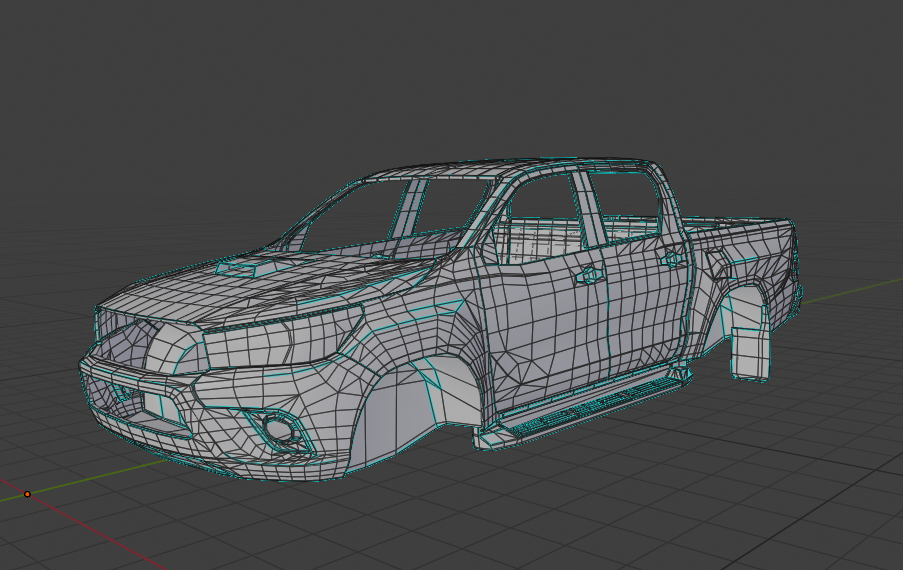
\includegraphics[width=\textwidth]{62.png}

  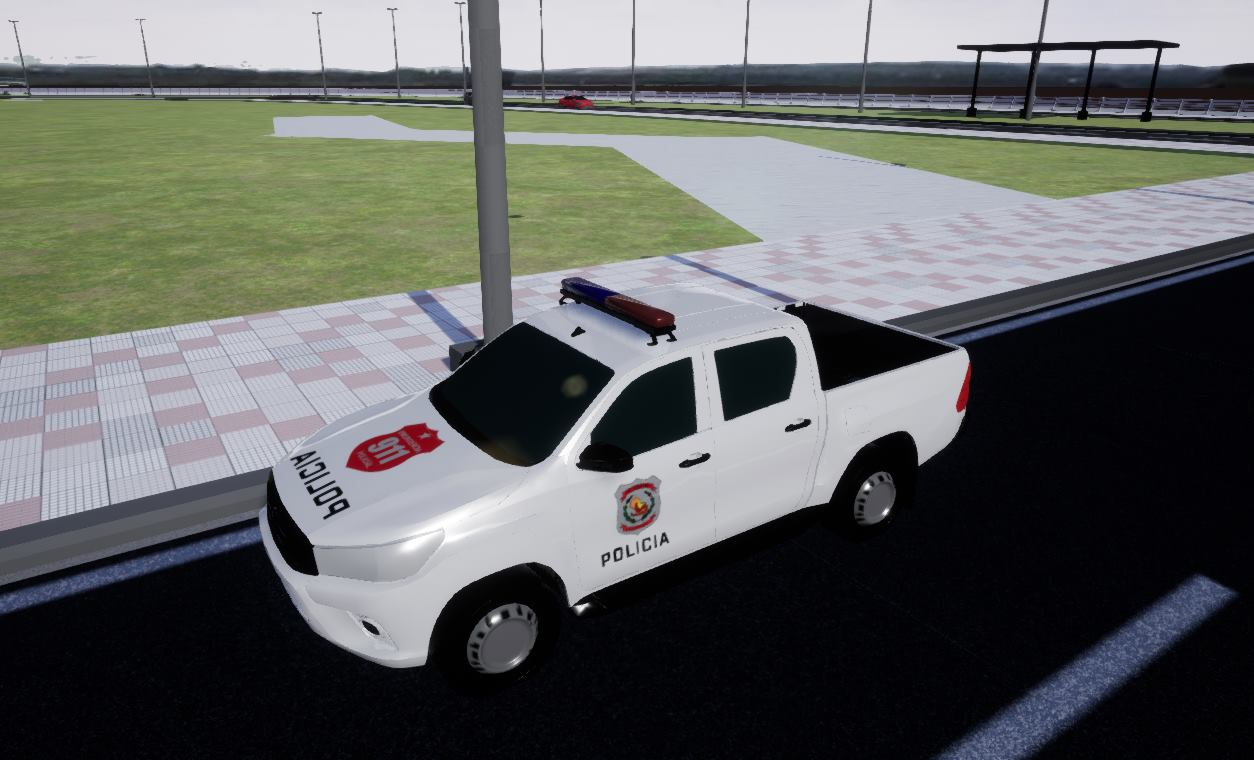
\includegraphics[width=\textwidth]{63.jpg}
  
  \includegraphics[width=\textwidth]{67.jpg}
  
  \includegraphics[width=\textwidth]{72.png}

  \includegraphics[width=\textwidth]{64.png}
  
  \includegraphics[width=\textwidth]{65.png}
  
  \includegraphics[width=\textwidth]{71.jpg}
  
  \includegraphics[width=\textwidth]{68.png}
  
  \includegraphics[width=\textwidth]{71.png}
  
  \includegraphics[width=\textwidth]{69.png}
  
  \includegraphics[width=\textwidth]{70.png}
  
  \includegraphics[width=\textwidth]{73.png}
  
  \includegraphics[width=\textwidth]{38.jpg}
  Now we have a police man character and police car
  
  \includegraphics[width=\textwidth]{57.jpg}
  I used the open source python project MetaHuman and a got an skin for the main character

  \includegraphics[width=\textwidth]{59.jpg}
  Eyes shaders need sometimes Heighmap 

  \includegraphics[width=\textwidth]{58.jpg}
  At some point you will want to test your model in a Game Engine, you can download a free city or some enviroment and test the model

  
  \includegraphics[width=\textwidth]{20.jpg}

  \includegraphics[width=\textwidth]{21.jpg}
  
  \includegraphics[width=\textwidth]{27.jpg}

  \includegraphics[width=\textwidth]{22.png}
  We can make a prototype user interface for selecting the character

  \subsection{Animation}
  \includegraphics[width=\textwidth]{30.png}
  
  \includegraphics[width=\textwidth]{31.png}
  I used skeletal bones for anim paraguayan bill

  \includegraphics[width=\textwidth]{28.png}

  \includegraphics[width=\textwidth]{29.png}
  
  \section{The Logic}

  https://github.com/pavonstudios/pavon-the-game-unreal

  \includegraphics[width=\textwidth]{46.jpg}

  -> Intel i7 4790K 4th Generation 8 cores
-> 16 GB RAM DDR3
-> NVIDIA GTX 1060 3GB
==>DVI Monitor
==>VGA to HDMI Monitor
->Integrated Graphics
==>VGA Monitor
Compile farm:
--->Intel Celeron 2 Core
--->Intel Dual Core
--->AMD E1-2500
Total Cores for GCC compiler: 12
Gentoo Linux like main operating system in all computer.

  \includegraphics[width=\textwidth]{47.jpg}

  \includegraphics[width=\textwidth]{48.png}

  \includegraphics[width=\textwidth]{49.jpg}

  \includegraphics[width=\textwidth]{50.png}

  \includegraphics[width=\textwidth]{51.png}
  
  \includegraphics[width=\textwidth]{52.png}

  \includegraphics[width=\textwidth]{53.png}

  \includegraphics[width=\textwidth]{55.png}

  \includegraphics[width=\textwidth]{54.png}
  


\end{document}
